\documentclass{article}
\usepackage[utf8]{inputenc}
\usepackage{amsfonts}
\usepackage{amsmath}
\renewcommand{\labelitemii}{$\circ$}
%% Custom commands
\newcommand{\E}[1]{\langle #1 \rangle} % shortcut for expectation
\newcommand{\norm}[3]{\mathcal{N}\left(#1; #2, #3\right)} %shorcut normal distributions
\newcommand{\imgwidth}{6in}
% \newcommand{\includeimage2}[1]{\includegraphics[width=6in]{#1}}
% \newcommand{\includeimage}[1]{\textbf{#1}}
% \newcommand{\bb}[1]{\mathbb{#1}}
\usepackage[final]{graphicx}
\graphicspath{ {./images/} }
\usepackage{subfigure}

\usepackage{longtable}
\usepackage{booktabs}
\usepackage{multirow}
\usepackage{array}
\usepackage[math]{cellspace}

\usepackage{geometry}

\usepackage{siunitx}
\usepackage{pifont}

\usepackage[version=4]{mhchem}

% \usepackage[a4paper, total={5in, 8in}]{geometry}

\usepackage{svg}

% make figure and tables captions bold
\usepackage[labelfont=bf]{caption}


% \let\Oldsubsubsection\subsubsection
% \renewcommand{\subsubsection}{\FloatBarrier\Oldsubsubsection}

\usepackage{sectsty}
\subparagraphfont{\itshape}


%%% hyperlinks into document
% see https://www.overleaf.com/learn/latex/Hyperlinks
\usepackage{hyperref}
\hypersetup{
    colorlinks=true,
    linkcolor=blue,
    filecolor=magenta,      
    urlcolor=cyan,
    citecolor=black,
    pdftitle={Master Thesis}
    }
    
%%% removeparagraph indent
\parindent=0pt

% \usepackage{titlesec}
% \titleformat*{\subparagraph}{\textit}

% --- colors
\usepackage{xcolor}
\definecolor{KFColor}{rgb}{27, 158, 119}
\definecolor{ERAColor}{rgb}{217, 95, 2}
\definecolor{MDSColor}{rgb}{117, 112, 179}
%%% === add support \subsubparagraph and \sssparagraph
% see https://tex.stackexchange.com/questions/94402/creating-a-subsubparagraph
% ---
\makeatletter
\newcounter{subsubparagraph}[subparagraph]
\renewcommand\thesubsubparagraph{%
  \thesubparagraph.\@arabic\c@subsubparagraph}
\newcommand\subsubparagraph{%
  \@startsection{subsubparagraph}    % counter
    {6}                              % level
    {\parindent}                     % indent
    {3.25ex \@plus 1ex \@minus .2ex} % beforeskip
    {-1em}                           % afterskip
    {\normalfont\normalsize\itshape\bfseries}}
\newcommand\l@subsubparagraph{\@dottedtocline{6}{10em}{5em}}
\newcommand{\subsubparagraphmark}[1]{}
\def\toclevel@subsubparagraph{6}
\makeatother
% ---
\makeatletter
\newcounter{sssparagraph}[sssparagraph]
\renewcommand\thesssparagraph{%
  \thesubsubparagraph.\@arabic\c@sssparagraph}
\newcommand\sssparagraph{%
  \@startsection{sssparagraph}    % counter
    {7}                              % level
    {\parindent}                     % indent
    {3.25ex \@plus 1ex \@minus .2ex} % beforeskip
    {-1em}                           % afterskip
    {\normalfont\normalsize\itshape}}
\newcommand\l@sssparagraph{\@dottedtocline{7}{10em}{5em}}
\newcommand{\sssparagraphmark}[1]{}
\def\toclevel@sssparagraph{6}
\makeatother

%%% ===

%% make sections floats barries
\usepackage{placeins}

\let\Oldsection\section
\renewcommand{\section}{\FloatBarrier\Oldsection}

\let\Oldsubsection\subsection
\renewcommand{\subsection}{\FloatBarrier\Oldsubsection}


\usepackage{siunitx}

\usepackage{listings}

\usepackage{biblatex}
\addbibresource{Thesis-references.bib}

\title{Evaluation of Kalman filter for meteorological time series imputation}
\author{Simone Massaro}
\date{February 2023}

\begin{document}


\begin{titlepage}
    \begin{center}
        \vspace*{1cm}
            
        \Huge
        \textbf{Evaluation of Kalman filter for meteorological time series imputation}
            
        \vspace{0.5cm}
        \LARGE
        % Thesis Subtitle
            
        \vspace{1.5cm}
            
        \textbf{Simone Massaro}
            
        \vfill
            
        Master Thesis\\
        Forest and Ecosystem Sciences
            
        \vspace{0.3cm}
            
        \Large
        Department Name\\
        Georg-August Universität Göttigen \\
        % Country\\
        February 2023
            
    \end{center}
\end{titlepage}
\clearpage
\tableofcontents
\clearpage
\section{Introduction}

\subsection{Eddy Covariance and gaps in meteorological variables}

Eddy Covariance (EC) is a state of the art technique for measuring green house gases and energy exchanges between ecosystems and the atmosphere \cite{aubinet_eddy_2012-1}.  The technique allows for non-destructive measurements at the ecosystem level with a high temporal resolution. Eddy Covariance data is used for ecological and physiological research of ecosystems, as well as for validation of ecosystem process models and remote sensing observations \cite{papale_ideas_2020}.
The core of Eddy Covariance site is the 3D anemometer and gas analysers, which allows estimating the fluxes of interests (e.g. \ce{CO_2}, \ce{H_2O}, \ce{CH_4}). Beside the fluxes, an Eddy Covariance setups collects measurements of meteorological variables and ecosystem parameters. This additional data provides the context to use and interpret the fluxes measurements.

\paragraph{} The acquisition of the meteorological variables can be interrupted by failures in the instruments or power outages, resulting in gaps in the time series \cite{aubinet_eddy_2012-1}.
The presence of gaps is a problem for several uses of the EC data.

An important application of EC is the validation of Land Surface Models \cite{balzarolo_evaluating_2014, friend_fluxnet_2007-1, bonan_improving_2011-1, kramer_evaluation_2002}, which are process based model that estimate fluxes using meteorological conditions as input. The errors of Land Surface Models deriving from inaccuracies in the input are comparable to the errors arising from the limitation in the models formulations \cite{zhao_how_2012}. This highlights the need of high quality continuous meteorological measurement that reflect that condition at the flux station.
Meteorological observations are used as a driver to impute gaps in the fluxes measurements \cite{aubinet_eddy_2012-1}, which requires complete meteorological time series.
Finally, the presence of gaps affects the calculation of long term averages for meteorological variables. 

\paragraph{} The described use cases make it necessary to impute the gaps in the meteorological variables. The first approach to reduce the number of gaps in to have redundant instruments on the site, however is this is not always possible and statistical models are used for imputing the gaps \cite{aubinet_eddy_2012-1}. There are three different approaches that can be used to reconstruct missing data: 1) use the \emph{temporal autocorrelation} of the variables, the measurements  before and after the gap provide information on the missing data; 2) use \emph{correlation} between different variables, if not all variables are missing the correlation between variables can be used for imputing the missing variable; 3) use \emph{other measurements}, meteorological variables not only measured in EC tower and the data from nearby meteorological stations can also be used for imputation.


\subsection{Current Imputation methods} EC post-processing pipeline impute meteorological time series. Arguably the most widely used post-processing pipeline is ONEFlux \cite{pastorello_fluxnet2015_2020}, which is adopted by FLUXENT, the global EC network, ICOS the European network as well as AmeriFlux, the American EC network.
ONEFlux uses two different methods for imputing the meteorological data: Marginal Distribution Sampling (MDS) and ERA-Interim (ERA-I). The final gap-filled meteorological product uses either MDS or ERA-I, depending on the quality flag of MDS.
\paragraph{MDS} Marginal Distribution Sampling \cite{reichstein_separation_2005-3} estimates the value of the missing variable by using the observations of the variable from other data points with similar meteorological conditions.
The algorithm finds all the similar conditions by taking the observations from a time window around the gap other meteorological variables have similar values in the gap.
All the observations of the variables of interest from similar conditions are then averaged to generate the filling value.
In case there are not similar meteorological conditions in the starting time window, the size of the time window is progressively increased. If other meteorological variables are also missing, they are not used to find similar conditions.

The algorithm implemented in ONEFlux uses as drivers the incoming shortwave radiation (\texttt{SW\_IN}), air temperature (\texttt{TA}) and Vapour pressure deficit (\texttt{VPD}). If \texttt{TA} or \texttt{VPD} is missing, \texttt{SW\_IN} is used as the only driver. If all drivers are missing, the mean value at the same of the day is used for gap filling. The starting size of the time window is 7 days.

MDS has a quality flag with 3 possible values (i.e. 1,2,3) that depends on the size of the time window. In ONEFlux MDS is used only if the quality flag is 1, which means that similar conditions are found in a time window smaller than 14 days.

\paragraph{ERA-Interim} ERA-Interim is a global meteorological dataset provided by the European Centre for Medium-range Weather Forecast (ECMWF). Weather forecast models are used to reanalyse past observations and produce a continuous and complete dataset for all the globe. The main drawback is the low spatial resolution and temporal resolution, that are respectively 0.7° (roughly 38\si{km}) and 3 hours. Moreover, only a subset of the meteoroligical variables are available in ERA-I. ONEFlux reduces the error of the ERA-I data by doing a bias correction with a linear regression and temporally downscaled to match the half-hourly frequency of FLUXNET \cite{vuichard_filling_2015}. 


\paragraph{Other methods} ONEFLux is not the only EC post-processing pipeline which gap fills meteorological data. However, the imputation approaches in other libraries, like REddyProc \cite{wutzler_basic_2018} or OzFlux \cite{isaac_ozflux_2017} are very similar. OzFlux implementation differs as it includes data from both ERA-Interim and the Australian Weather Service and for each gaps select the dataset with the smallest error for a window of 90 days around the gap.
\pagebreak
\paragraph{Limitations of current methods} There are three possible direction to improve the current imputation methods  1) make a better use of temporal autocorrelation of the variables 2) combine different imputation approaches in one prediction  3) provide detailed information on the quality of imputation.

\subparagraph{Temporal autocorrelation} MDS uses the temporal autocorrelation only in a limited way, as it takes the average of the missing variable across the whole time window and doesn't attribute more weight to the observations closes to the gap, which have the highest correlation with the data in the gap. This is especially relevant for short and medium gaps, which are the majority of gaps in FLUXNET (Appendix figure \ref{fig:gap_len_dist}). The bias correction for ERA-Interim doesn't take into consideration the observations around the gap, either. Therefore, there is potential in improving the imputation performance by making a better use of the temporal autocorrelation.

\subparagraph{Combination of imputation approaches} ONEFlux employs both ERA-I and MDS, but the two methods are used independently, not combined to improve the predictions, but they are used independently. The criteria to select the method to use is only the MDS quality control flags. The information on the missing data from temporal autocorrelation, correlation with other variables and other measurements can be combined to make one more accurate prediction.

\subparagraph{Uncertainty} A limitation of the current methods is the lack of a robust assessment of the uncertainty of the imputed values. MDS has a quality flag, but it derives from hardcoded values and has only 3 possible values, moreover in the final ONEFlux product the quality flag indicates only which gap filling method has been used. Ideally, each predicted data point has an associated uncertainty, which varies continuously and it is interpretable. In this way, the level of confidence of the model in each prediction is available to the data user. The uncertainty can be used either to discard the data above a custom threshold, which can change depending on the application, or directly included in the downstream calculations.

\subsection{Kalman Filter}
Imputation of missing values is a topic that has been extensively researched. A wide range of methods have been developed ranging from replacing with the mean to employing deep neural networks \cite{fang_time_2020-1, buuren_mice_2011, du_saits_2022-1, zhang_dual-head_2021-2, cao_brits_nodate}. Specifically for meteorological time series there are many different methods \cite{costa_gap_2021, jing_multi-imputation_2022}. However, imputation in the EC contest has some specific characteristics: the absence of a spatial component (each EC site is modelled separately) and the relatively high number of variables. Moreover, the focus is to impute short and medium gaps (up to 1 week), as almost 99 \% of gaps of meteorological variables in FLUXNET are shorter than a week (Appendix figure \ref{fig:gap_len_dist}). For this work, we focused into methods that combine all imputation approaches, include interpretable uncertainty and can be applied globally. 
% In the EC the focus is to impute gaps into fluxes measurements, as the number of missing observations is very high (), however the meteorological 
% there are many different approaches for time series imputation and for  ().
% [fluxes gap filling, deep learning ]
% However, of meteorological variables imputation for EC has some specific requirements and conditions. To enhance the quality of the imputation  the models should include all the three point mentioned above: 1) use effectively variable autocorrelation 2) combining autocorrelation, variable correlation and other measurements in one prediction 3) provide an interpretable uncertainty for each prediction. The gap filling in this setting has also two important advantages: the availability of other measurements (e.g. ERA-I) and the fact that the majority of the gaps are not long, which simplifies the complexity of the model.
\paragraph{} There are many families of models that can be suitable for the task. Probabilistic machine learning algorithms are particularly suited, as they directly provide an interpretability uncertainty.
Kalman Filter is a probabilistic model that models the evolution of a multivariate latent state over time using a Markov chain. The temporal autocorrelation and the variable correlation are directly considered by the model and is possible to also include ERA-I observations.
Other modelling approaches were evaluated: Gaussian Process Factor Analysis and GP-VAE (Gaussian Processes Variational AutoEncoders). Gaussian Processes Factor Analysis \cite{yu_gaussian-process_2008} use Gaussian Processes to model a latent variable over time, this is a powerful modelling approach and is fully probabilist. The main limitation is the computational complexity, which in the naive formulation scales cubically with the number of observations.
GP-VAE \cite{fortuin_gp-vae_2020} combines Gaussian Processes and deep learning, to provide high quality imputation with uncertainties.
Kalman Filter was selected, since it's the simplest model of the one considered that still fulfils all the requirements.
% \begin{itemize}
% \item need to find a modelling approach that can meet those requirements
% \item combine 3 gap filling approaches
% \item provide uncertanties
% \item by analyzing the gap length in Fluxnet for meteo variables the gaps are short (see Appendix )
% \item there are many possible approaches (eg. GP-VAE, random forests)
% \item so we likely don't need a very complex model
% \item kalman filter is on of the simplest model that can fit the requirements
% \end{itemize}

\paragraph{} The first goal of this work is to develop an imputation method for meteorological time series in the context of EC that employs a Kalman Filter. The imputation performance of the new method is then evaluated by comparing it with the state-of-the-art methods (ERA-I and MDS) and assessing the behaviour in different scenarios. For simplicity, only data from one EC site, Hainich (Germany), will be used.


\section{Methods}

\subsection{Kalman Filter Theory}

Kalman Filter models over time a latent variable $x$, that represent the state of the system. The state cannot be directly observed, but we can observe meteorological variables $y$ that reflect the state of the system. It is possible to use Kalman Filters to impute missing values, as the value of the state can be updated over time even when there are missing observations. The values of the state are hence available for all time steps, which can be used to then predict the missing observed variables.
Kalman Filter is a probabilist machine learning algorithms, so it keeps track of the entire distribution of the latent state $p(x_t)$. The time is considered to be discrete, the state is modelled only at specific times $x_t$.  

\paragraph{} In order to be to model the state over time, assumptions on the behaviour of the system are made. There are three key assumptions 1) the states are connected by a Markov chain, which means that the state at time $t$ depends only on the state at time $t-1$ and not the states at previous times $p(x_t|x_{t-1}) = p(x_t|x_{t-1}, x_{t-2}, \hdots, x_0)$ 2) The value of the observed variable depends on the latent state 3) all the relationships are linear and all distributions are Gaussian. Additionally, the mean of the state at time $t$ may depend also on an external control variable. This control variable doesn't depend on the state of the models, but provide information on how the state mean should change.
Equations \ref{eq:system_state} and \ref{eq:system_obs} describe the assumptions on the behaviour of the system:

\begin{align}
p(x_t | x_{t-1}) &= \norm{x_t}{Ax_{t-1} + b + Bc}{Q} \label{eq:system_state}\\
p(y_t | x_t) &= \norm{y_t}{Hx_t + d}{R} \label{eq:system_obs}
\end{align}

The probability distributions of the state are computed using Bayesian inference. The computational cost of probabilistic inference can be drastically reduced in this context, since all the relations are linear and all distributions are Gaussian, which means that probabilistic inference can be performed using linear algebra operations.

\paragraph{} Kalman Filter is a recursive algorithm (Figure \ref{fig:kalman_filter}), at time $t$ the \textit{predicted state} ($x^-_t$) is obtained from the previous state ($x_{t-1}$) and the \textit{control variable} ($c_t$). Then the state is update using the \textit{observation} ($y_t$) to obtain the \textit{filtered state}, observations can be partially or totally missing. This is repeated recursively for all time steps. At this point, each time step, the state $x_t$ depends only on the observations until time $t$. The \textit{smoothed state} ($x^s_t$) is the final state that depends also on all the observations after time $t$. The smoothing phase works by starting from the last time step and recursively updating $x^s_t$ using $x^s_{t+1}$, $x_{t+1}$ and $x^-_{t+1}$.
Finally, for all the time steps where there is a gap, the \textit{predicted observations}, $\hat{y}^g_t$, are calculated from the state $x_t$.

The model always considers the probability distribution for the state ($p(x_t) = \norm{x_t}{m_t}{P_t}$), for each state at each time step the mean ($m_t$) and the covariance are ($P_t$) are stored that are the parameters for a multivariate Gaussian distribution. Similarly, the model predictions are a distribution $p(\hat{y}_t) \norm{\hat{y_t}}{\mu_{y_t}}{\Sigma_{y_t}}$.

\begin{figure}
\includegraphics[width=\textwidth]{Kalman Filter figure.png}
\caption{Schematic representation of a Kalman Filter}
\label{fig:kalman_filter}
\end{figure}

\subsubsection{Time update}

The first step in a Kalman Filter is computing the probability distribution of the predicted state $x^-_t$, from the state at the previous time step $x_{t-1}$ and the control variable $c_t$. The predicted state distribution is $p(x_{t-1}) = \mathcal{N}(m_{t-1}, P_{t-1})$.  Using equation \ref{eq:system_state} and the properties of a linear map of Gaussian distributions the following equation can be derived:

\begin{align}\label{eq:time_update}
    p(x^-_t) &= \norm{x_t^-}{m_t^-}{ P_t^-}\\
    m_t^- &= Am_{t-1} + B c_t + d \label{eq:time_update_mean}\\
    P_t^- &= AP_{t-1}A^T + Q \label{eq:time_update_cov}
\end{align} 

\subsubsection{Measurement update}

The predicted probability distribution is the updated to obtain the distribution of the filtered state, using the current observation ($y_t$). Equation \ref{eq:system_obs} describes the distribution of $y_t$ given $x_t$, but using Bayes theorem is possible to compute the distribution of $x_t$ given an observation $y_t$.

\begin{align}
 p(x_t|y_t) &= \mathcal{N}(x_t; m_t, P_t) \label{eq:meas_update}\\
 z_t &= Hm_t^- + d \label{eq:meas_update:obs_mean}\\
 S_t &= HP_t^-H^T + R \label{eq:meas_update:obs_cov}\\
 K_t &= P_t^-H^TS_t^{-1} \label{eq:meas_update:kalman_gain}\\
 m_t &= m_t^- + K_t(y_t - z_t) \label{eq:meas_update:state_mean}\\
 P_t &= (I-K_tH)P_t^- \label{eq:meas_update:state_cov}
\end{align}
    
\paragraph{Missing observations}

The Kalman Filter is robust to missing data and can update the state even though there is missing data. 
If all the observations at time $t$ are missing, the measurement update step is skipped and the filtered ($x_t$) is the same of the predicted state ($x_t^-$). If only some observations in $y_t$ are missing, then a partial measurement step is performed.
The vector containing the observations that are not missing at time $t$, $y^{ng}_t$, can be expressed as a linear transformation of $y_t$

\begin{equation}\label{eq:miss_obs}
    y^{ng}_t = My_t
\end{equation}

where $M$ is a mask matrix that is used to select the subset of $y_t$ that is observed. $M \in \mathbb{R}^{n^{ng} \times n}$ and is made of rows which are made of all zeros but for an entry 1 at column corresponding to the of the index of the non-missing observation.

For example, if $y_t = [y_{0,t}, y_{1,t}, y_{2,t}]^T$ and $y_{0,t}$ is the missing observation then

\begin{equation}
 M = \left[\begin{array}{ccc}
    0 & 1 & 0 \\
    0 & 0 & 1
\end{array}\right]
\end{equation}

 using the properties of linear projections of Gaussian distribution we can then derive the distribution $p(y^{ng}_t \mid y_t)$ and from it $p(y^{ng}_t \mid x_t)$ 

\begin{align}
   p(y^{ng}_t|y_t) &= \norm{y^{ng}_t}{M\mu_{y_t}}{M\Sigma_{y_t}M^T} \label{eq:partial_obs}\\
  p(y^{ng}_t|x_t) &= \norm{y^{ng}_t}{MHx_t + Mb}{MRM^T}\label{eq:partial_obs_state}
\end{align}

Therefore, it is possible to perform the measurement update step when some observations are missing using a variation of equation \ref{eq:meas_update}, where $H$ is replaced by $MH$, $b$ by $Mb$ and $R$ by $MRM^T$.

\subsubsection{Smoothing}

In the smoothing step, the filtered state at time $t$ is update using the state ${t+1}$ corrected by the measurement update. A set of equations for the smoothing pass of a Kalman Filter has been derived by Rauch-Tung-Striebel. They calculate the smoothed state $x_t^s$ from the smoothed, filtered and predicted state at the successive time step.
For the last time step, the smoothed state is set to be equal to the filtered state.

\begin{align}
    p(x_t^s \mid Y) &= \norm{x_t^s}{m_t^s}{P_t^s} \label{eq:smoother}\\
    G_t &= P_tA^T(P_{t+1}^-)^{-1} \label{eq:smoother:gain}\\
    m_t^s &= m_t + G_t(m_{t+1}^s - m_{t+1}^-) \label{eq:smoother:mean}\\
    P_t^s &= P_t + G_t(P_{t+1}^s - P_{t+1}^-)G_t^T \label{eq:smoother:cov}
\end{align}

\subsubsection{Predictions}

From the state ($x_t$) it is possible to directly obtain the predictions of the model $\hat{y}^g_t$ by using equation \ref{eq:system_obs} and a mask as described in equation \ref{eq:miss_obs}

\begin{align}\label{filter_predictions}
    p(\hat{y}^g_t) &= \norm{\hat{y}^g_t}{\mu_{y_t}}{\Sigma_t} \\
    \mu_{y_t} &= MHx_t + Md \\
    \Sigma_{y_t} &= MRM + MHP^s_tH^TM^T
\end{align}


\subsection{Kalman Filter Implementation}

\subsubsection{Requirements}

Kalman Filter are a widely used algorithm and there are several python libraries that implement Kalman Filter (e.g. \verb|statsmodels|, \verb|pykalman|, \verb|filterpy|). However, the application of Kalman Filters in this context  we didn't manage to identify a library that meets all the requirement: support gaps and partial measurements updates, use log likelihood for maximization and use a numerically stable implementation of the smoother.

support control variable

Therefore a custom library for Kalman Filters was developed using the PyTorch library, which has the advantage of automatic differentiation, possibility to use GPUs and better integration with other Machine Learning methods.

\subsubsection{Numerical stability}

\paragraph{Background}
The direct implementation of the Kalman filter equations suffer by numerically stability issues \cite{mohinder_s_grewal_kalman_2001, dan_simon_optimal_2006}, hence several techniques have been developed to mitigate this.

Numerical instability arises from the fact that digital computers store numbers only with a limited number of decimal digits, which results in a loss of information, so that some operations may be incorrectly performed by a  computer (e.g. summing a big number and a small number).

For Kalman Filter the components that are most affect by numerically instability are the covariance matrices. To analyse the stability of the operations on these matrices it is relevant to consider the condition number for inversion \cite{mohinder_s_grewal_kalman_2001, kaminski_discrete_1971}, which describes if the matrix is going to be singular on the numerical representation in the computer and thus cannot be inverted. The condition number ($k(A)$) is the ratio between the biggest singular value ($\sigma(A)$). $\sigma^2(A) = \lambda(AA^T)$, with  $\lambda(A)$ being the eigenvalue of $A$
\begin{equation}\label{condition_number}
    k(A) = \frac{\sigma_{max}(A)}{\sigma_{min}(A)}
\end{equation}

The condition number it's 1 for well-conditioned matrices and tends to infinite for ill-conditioned matrices. As a general rule  a matrix cannot be inverted when the reciprocal of the condition number for inversion is close to the machine precision $ 1/k(A) < \varepsilon$ \cite{mohinder_s_grewal_kalman_2001}.

\paragraph{Mitigation strategies}

\subparagraph{Machine precision} The simplest to improve the numerical stability is to use higher accuracy in the representation of numbers \cite{dan_simon_optimal_2006}. Practically, this means to use 64bit floats instead of 32bit floats, which is default in PyTorch.

\subparagraph{Matrix decomposition} Another way to improve the numerical stability is to reduce the condition number of the matrices, for the Kalman filter the key matrix is the state covariance ($P$). A positive definite matrix has a square root factor, $P^{1/2}$, such as that $P = P^{1/2}(P^{1/2})^T$. If the store $P^{1/2}$ instead of $P$ the effective numerical resolution of the filter can be doubled \cite{kaminski_discrete_1971} \cite{dan_simon_optimal_2006} \cite{rutten_square-root_2013}. This is due to the fact that the eigenvalues of $P^{1/2}$ are the square root of the eigenvalues of $P$ ($\lambda(P) = \lambda^2(P^{1/2})$), thus the conditioning number of $P$ is the square of the conditioning number of $P^{1/2}$, which results in practically doubled. Therefore, if in the filter implementation $P$ is never explicitly computed, the numerical stability of the filter is significantly improved.
There are several approached of filter implementations that follow this approach (\cite{potter_statistical_1963}, \cite{carlson_fast_1973}, \cite{bierman_numerical_1977}) and are generally called ``square-root filter''. Different implementat which have different tradeoff and often are computationally more expensive that the conventional implementation 

\subsubsection{Implementation in PyTorch}

There are different approaches for square root filtering. According to \cite{mohinder_s_grewal_kalman_2001} the best approach is the UD Filter (\cite{bierman_numerical_1977}), since it has the smallest computational cost. However, the filter is based on the $UD$ factorization and a custom matrix factorization \cite{mohinder_s_grewal_kalman_2001} and both of those algorithms cannot be efficiently implemented in PyTorch. The PyTorch function \verb|torch.linalg.ldl_factor| performs an $UD$ factorization, but it's an experimental function and is not differentiable. Moreover, the custom matrix factorization would need to be implemented using scalar operations, which aren't efficient with PyTorch eager execution.

For this reason, a square root filter that propagates Cholesky factors of the covariance matrices is implemented. In this way all the required computations can be expressed in QR factorization, which is a numerically stable method and is a routine implemented in PyTorch.

\subsubsection{Time update Square Root Filter}

The equations for the time update step of the filter are from \cite{mohinder_s_grewal_kalman_2001} eq. 6.60.

For notation simplicity, we define $P_t=P_t^{1/2}P_t^{T/2}$ where $P_t^{1/2}$ is lower triangular matrix, and $P_t^{T/2} = (P_t^{1/2})^T$. In the same way, $Q=Q^{1/2}Q^{T/2}$. In the Kalman filter literature $P_t^{1/2}$, is the ``square root'' of $P_t$, hence the name of this type of filter. The Cholesky decomposition is an algorithm to find a square root of a matrix, however the Cholesky decomposition calculates only one of possibly many square roots of the matrix. In fact, $P_t^{1/2}$ is not unique.

The goal is to derive from the equations of prediction step (eq. \ref{filter_predict}) an algorithm to obtain $P_t^{1/2}$ given $P_{t-1}^{1/2}$, without explicitly computing $P_t$ or $P_{t-1}$. In this way, the numerical stability of the model is effectively doubled.

If we define

\begin{equation}
    W = \begin{bmatrix}AP_{t-1}^{1/2} & Q^{1/2}\end{bmatrix}
\end{equation}

then using \ref{filter_predict} we can prove that
\begin{equation}\label{predict_SR_mult}
WW^T = P_t 
\end{equation}

\begin{multline}
  WW^T =  \begin{bmatrix}AP_{t-1}^{1/2} & Q^{1/2}\end{bmatrix}\begin{bmatrix}P_{t-1}^{T/2}A^T \\ Q^{T/2}\end{bmatrix}\\
  = AP_{t-1}^{1/2}P_{t-1}^{T/2}A^T + Q^{1/2}Q^{T/2} = AP_{t-1}A^T + Q = P_t
\end{multline}

If we  can factorize $W=LU$, where $L$ is a lower triangular matrix and $U$ is an orthogonal matrix, such as that $UU^T = I$. Then $WW^T = LU(LU)^T = LUU^TL^T = LL^T$ and by equation \ref{predict_SR_mult} $LL^T=P_t$. Hence, $L$ is a square root of $P_t$, which is what we were looking for.

This procedure never explicitly compute $P_t$ and requires only the factorization of a matrix, which is implemented efficiently and in a numerical stable way by PyTorch \verb|torch.linalg.qr| function. 

\subparagraph{PyTorch implementation} PyTorch doesn't support natively a $LU$ decompositions. It implements the QR factorization: $W=QR$, where $Q$ is an orthogonal matrix and $R$ an upper triangular matrix. This can be easily converted into a $LU$ factorization, since by factorizing $W^T$ then $W^=QR=(QR^T)=R^TQ^T$ and $R^T$ is a lower triangular matrix.

\subparagraph{Summary} The steps of the Square Root time update are:

\begin{enumerate}
    \item let  $W = \begin{bmatrix}AP_{t-1}^{1/2} & Q^{1/2}\end{bmatrix}$
    \item do a QR factorization $W^T=TR$
    \item define $P_t^{1/2} = R^T$
\end{enumerate}

\subsubsection{Measurement update Square Root Filter}

A similar procedure can be followed for the measurement update step of the filter. The equations here described are from \cite{dan_simon_optimal_2006}.

The starting point is equation \ref{filter_update} and for simplicity the time subscript are omitted in the following equations

Letting:

\begin{align}
    M &= \begin{bmatrix} R^{1/2} & H(P^-)^{1/2} \\ 0 & (P^-)^{1/2} \end{bmatrix} \\
    V &= \begin{bmatrix} S^{1/2} & 0 \\ \bar{K} & P^{1/2} \end{bmatrix} \\
    \bar{K} &= KS^{1/2}
\end{align}
    
Then we can prove that 

\begin{equation}\label{update_SR_mult}
    MM^T = UU^T
\end{equation}

Therefore, if we decompose $M=LU$ then $LL^T=UU^T$ and the bottom left block of size $k \times k$ of $L$ is a square root of $P$.

Here we prove equation \ref{update_SR_mult}

\begin{equation}
\begin{split}
    MM^T &= \begin{bmatrix} R^{1/2} & HP^- \\ 0 & (P^-)^{1/2} \end{bmatrix}\begin{bmatrix} R^{T/2} & 0 \\ (P^-)^{T/2}H^T & (P^-)^{T/2} \end{bmatrix}= \\
    &=\begin{bmatrix} R^{1/2}R^{T/2} + H(P^-)^{1/2}(P^-)^{T/2}H^T & HP^-)^{1/2}P^-)^{T/2} \\ (P^-)^{T/2}P^-)^{1/2}H^T & (P^-)^{1/2}P^-)^{T/2} \end{bmatrix} = \\
    &=\begin{bmatrix}S & HP^- \\ (P^-)^TH^T & P^- \end{bmatrix}
\end{split}
\end{equation}

\begin{equation}
\begin{split}
VV^T & = \begin{bmatrix} S^{1/2} & 0 \\ \bar{K} & P^{1/2} \end{bmatrix}\begin{bmatrix} S^{T/2} & \bar{K}^T \\ 0 & P^{T/2} \end{bmatrix} = \begin{bmatrix} S^{1/2}S^{T/2} & S^{1/2}\bar{K}^T \\ \bar{K}S^{T/2} & \bar{K}\bar{K}^T + P^{1/2}P^{T/2} \end{bmatrix}\\
 & = \begin{bmatrix} S & S^{1/2}S^{T/2}K^T \\ KS^{1/2}S^{T/2} & KS^{1/2}S^{T/2}K^T + P\end{bmatrix} \\
 & = \begin{bmatrix} S & HP^- \\ P^-H^T & KHP + P\end{bmatrix} \\
\end{split}
\end{equation}

We can see that all blocks of $VV^T$ are directly equal to $MM^T$, but the bottom left one, which is equal due to the measurement update for the covariance (equation \ref{eq:meas_update:state_cov}).

\subparagraph{Summary} The steps of the Square Root measurement update are:
\begin{enumerate}
 \item let $M = \begin{bmatrix} R^{1/2} & H(P^-)^{1/2} \\ 0 & (P^-)^{1/2} \end{bmatrix}$
 \item do a QR factorization of $M^T=TV$
 \item $P^{1/2}$ is the bottom left $k \times k$ block of $V^T$
\end{enumerate}

\subsubsection{Predictions Square Root Filter}

The prediction equation for the square root filter are similar to the equations for the time update.

We define:

\begin{equation}
    W = \begin{bmatrix}HP_{t}^{1/2} & R^{1/2}\end{bmatrix}
\end{equation}

then using equation \ref{filter_predict} we can prove that
\begin{equation}\label{predict_SR_mult}
WW^T = O_t 
\end{equation}

\begin{multline}
  WW^T =  \begin{bmatrix}AP_{t}^{1/2} & R^{1/2}\end{bmatrix}\begin{bmatrix}P_{t}^{T/2}H^T \\ R^{T/2}\end{bmatrix}\\
  = HP_{t}^{1/2}P_{t}^{T/2}H^T + R^{1/2}R^{T/2} = HP_{t}H^T + R = O_t
\end{multline}

\subparagraph{Summary} The steps of the Square Root predictions are:

\begin{enumerate}
    \item let  $W = \begin{bmatrix}HP_t^{1/2} & R^{1/2}\end{bmatrix}$
    \item do a QR factorization of $W^T=TU$
    \item define $\Sigma_{y_t}^{1/2} = U^T$
\end{enumerate}

\subsubsection{Smoother}

The available literature for implementing Square Root Smoothing is scarce compared to Square root filter, so no solution has been identified to implement a square root smoother. Therefore, a standard smoother is employed.
Nonetheless, steps were taken to improve the numerical stability of the smoother. The computation in the smoother that is most numerically unstable is the inversion of $P^-_{t+1}$ in equation \ref{eq:smoother:gain}. The direct matrix inversion is avoided by using the \verb|torch.cholesky_solve| function, which solves for $X$ the linear system $P^-_{t+1}X=P_tA$, which is equivalent of computing $X = (P_tA^T(P^-_{t+1})^-1)^T$. This use directly the Cholesky Factor $(P^-_{t+1})^{1/2}$ to avoid the computation of $P^-_{t+1}$. A further step to improve the numerical stability is forcing the covariance matrix to be symmetric, by averaging to upper and lower part at after every time step $P^s_{t, sym} = (P^s_t + (P^s_t)^T)/2$, as suggested in \cite{dan_simon_optimal_2006}.
This approach to numerical stability in the smoother is the same implemented in state of the art libraries, such as `statsmodels`.

\subsection{Model}

\subsubsection{Parameters}

\begin{table}
\caption{Parameters of the Kalman Filter Model. $n$ is the number of dimension of the observations, $k$ the number of dimensions of the state, $n_{ctr}$ the number of dimensions of the control variable.}
\label{table:parameters}
\vspace{5pt}
\centering
\begin{tabular}{l c c c}
\toprule
    \bfseries Parameter name & \bfseries Notation & \bfseries Shape & \bfseries Initial value\\
    \hline
    \noalign{\vspace{4pt}}
    State transition matrix & $A$ & $k \times k$ & $\begin{bmatrix}I & I \\ 0 & I\end{bmatrix}$ \\
    \noalign{\vspace{4pt}}
    Observation matrix & $H$ & $n \times k$ & $\begin{bmatrix}\Lambda & 0 \end{bmatrix}$ \\
    State transition covariance & $Q$ & $k \times k$ & $0.1 I$ \\
    Observation covariance & $R$ & $n \times n$ & $0.01 I$\\
    State transition offset & $d$ & $k$ & 0 \\
    Observation offset & $b$ & $n$ & 0 \\
    Control matrix & $B$ & $k \times n_{ctr}$ & $\begin{bmatrix} -I & I \\ 0 & 0 \end{bmatrix}$ \\
    Initial state mean & $m_0$ & $k$ & $0$ \\
    Initial state covariance & $P_0$ & $k \times k$ & $3 I$ \\
\bottomrule
\end{tabular}
\end{table}

The Kalman Filter is implemented as PyTorch module, whose parameters are described in Table \ref{table:parameters}.
There is no change over time of the parameters, and the state of the filter is initialized always at the same value from the parameters $m_0$ and $P_0$.

\paragraph{Constraint}

An important aspect for implementing a Kalman Filter in PyTorch is constraining the parameters that represents covariance ($Q$, $R$ and $P0$) to be positive definite. To achieve this goal the optimizer works on a raw parameter, which is then transformed into a positive definite matrix.
The transformation into a positive definite matrix is done by transforming the raw parameter into a lower triangular matrix with a positive diagonal. The diagonal is enforced to be positive by transforming the diagonal of the raw parameter with the softplus function (eq. \ref{softplus}), which is positive function. In addition to the diagonal a small offset $\num{1e-5}$ is added to avoid that the diagonal is close to zero, which would result in positive semi-definite matrix.

\begin{equation}\label{softplus}
    x = \log (1 + e^{x})
\end{equation}

The inverse of the positive definite transformation is implemented, so that parameters can be manually set.

This implementation of the positive definite constraint makes it is that is straightforward to obtain the Cholesky factor of the parameters, which are needed by the Square Root Filter, and at the same time the full parameter, which are needed by the smoother.

\subsubsection{Parameters initialization}

The model parameters could be initialized using random values, however this would increase numerical stability issues and increase the training time. Moreover, if the initial parameters are very distant from the optimal one the optimization algorithm would find a local minimum, which is not the global minimum.  The simplicity of the Kalman Filter and the interpretability of its parameters allows to manually initialize the parameters with realist values.

\paragraph{State transition matrix} $A$ is initialized using a ``local linear trend'' model \cite{durbin_time_2012}. The idea of a local slope model is that half of the state $x_{l_{t-1}}$ represent the level of the current state and the second half the slope $x_{s_{t-1}}$ of a linear function that describes the rate of change of the state between time steps. The next state level is equal to the current level plus the slope and a random change, while the slope remains constant. In this way, the model can also keep track of the previous states.

\paragraph{Observation Matrix} $H$ is initialized by using the transpose of the factor loadings matrix of the principal component analysis. This is done to have a latent variable to represent the state between different variables, so that in the presence of a gap. The second part is 0 as in a local trend model the observations don't depend on the slope but only the level of the state

\paragraph{Control matrix} $B$ is initialized to the difference between the previous observation and the current observation. The number of dimensions of the control is potentially different from the state and the observations, therefore is difficult to find a proper correspondence between the state and the control. The solution found is to initialize the upper part of the matrix to the difference between the control, which roughly correspond to the variables and then pad the rest with zero to match the correct shape.

\paragraph{Covariance} The state transition covariance $Q$ and then observation covariance $R$ are initialized as diagonal matrix with values of $0.1$ and $0.01$ respectively. This number has been chosen to represent an uncertainty in the state transition that is compatible with standardized variables  and low uncertainty in the observations. 

\paragraph{Offsets} The observation and state transition offsets are initialized to zero.

\paragraph{Initial state} The initial state is set to a zero mean and as covariance a matrix with 3 on the diagonal. The number 3 is an arbitrary number significantly bigger than the state transition covariance, which should represent the high level of uncertainty for the initial state.  

\subsubsection{Loss Function}

The loss function is used to train the model is the negative log likelihood, computed for each data point. At each time step the model predicts a multivariate normal distribution $p(\hat{y}^g_t)$, which is used to compute the negative log likelihood given the actual observations $y_t^g$. The negative log likelihoods between different time steps in the same gaps are summed. Then negative log likelihood is averaged between batches.

The actual loss function of the model should be the log likelihood of the joint distribution $p(Y^g)$. However, the analytical form of the joint distribution cannot to easily derived from the Kalman Filter equations and the sum of the log likelihood of marginal distributions is a lower bound to the log likelihood of the joint distribution. If we define $q(x)$ the predicted joint distribution, $p(x)$ the real joint distribution and $q_i(x)$ the marginal distribution at the \textit{i}th time step
\begin{equation}
    q_i(x) = \int q(x_1, ..., x_k)dx_{\neg i}
\end{equation}

Then, if the family of distribution of $q(x \mid \theta)$, where $\theta$ are the model parameters, is the same of $\prod_i q_i(x \mid \theta)$ then

\begin{equation}\label{eq:log_joint_geq}
    \max_\theta \E{\log q(x\mid \theta)}_{x \sim p(x)} \geq \max_\theta \E{\log \prod_i q_i(x\mid \theta)}_{x \sim p(x)}
\end{equation}

because $\prod_i q_i(x)$ is more restricted. This means that $q(x)$ can fit at least as good as $\prod_i q_i(x)$.
For the Kalman Filter $q_i(x)$ is a Gaussian distribution, so $\prod_i q_i(x)$ is also a Gaussian distribution and equation \ref{eq:log_joint_geq} is true. The conclusion is that if we can fit the model by maximizing the sum of the log likelihoods at each time steps.

\subsubsection{Metrics}

The main metric used to assess the model performance is the Root Mean Square Error (RMSE). 

\begin{equation}
    RMSE = \sqrt{\frac{\sum_i^n (y^g_i - \hat{y}^g_i)^2}{n}}
\end{equation}

The advantages of the RMSE is that can be used for non-probabilistic methods (e.g. MDS) and that it's value has the same physical dimension of the observed variable. The main drawback is that is cannot be used for comparison between variables, for that the standardized RMSE is used, which is the RMSE computed on the standardized variables.

\subsubsection{Performance considerations} 

The iterative nature of the filter, where the current state depends on the previous state, makes it impossible to use PyTorch vectorization across different time steps. This can significantly limit the performance of the filter, especially when executed on GPUs. In order to  mitigate this issue, all functions in the Kalman Filter library support batches, so at every time step different data is processed in parallel.


\subsection{Data}

\subsubsection{Data source}

The data used to evaluate the performance of Kalman Filters is from the Hainich (Germany) site, which is managed by the University of Göttingen. The source of the data is  the FLUXNET 2015 Dataset, which includes measurements with a 30 mins frequency between 2000 and 2012 for Hainich. In total 227952 observations are available. For simplicity the entire dataset was used for the model training, which includes also gap-filled observations.
All the meteorological variables that are gap-filled in the FLUXNET 2015 dataset were selected for the analysis (Table \ref{table:variables}).

\paragraph{ERA-Interim} The control variables used in the Kalman Filter are the bias corrected and downscaled ERA-I observations included in the FLUXNET dataset. The variables of interest are also present in ERA-I, except for TS and SWC.

\paragraph{Gap distribution}The entire FLUXNET 2015 dataset was used to compute the distribution of gap lengths across the all the sites for each variable. A gap was definite when the QC flag of the variable is different from 0 or the data itself is missing (Appendix figure \ref{fig:gap_len_dist}).

\begin{table}
\caption{Meteorological variables used to evaluate the Kalman Filter imputation. ERA-I column indicates whether the variable is available in the ERA-Interim dataset}
\label{table:variables}
\vspace{5pt}
\centering
\begin{tabular}{l>{\bfseries}llc}
\toprule
    \bfseries Variable Name & \bfseries Abbreviation & \bfseries Unit & \bfseries ERA-I \\
    \hline
    Air Temperature & \lstinline|TA| & \si{^{\circ}C} & \ding{51}\\
    Incoming Shortwave Radiation & \lstinline|SW_IN| & \si{W/m^2} & \ding{51}\\
    Incoming Longwave Radiation & \lstinline|LW_IN| & \si{W/m^2} & \ding{51}\\
    Vapour Pressure Deficit & \lstinline|VPD| & \si{hPa} & \ding{51}\\
    Wind Speed & \lstinline|WS| & \si{m/s} & \ding{51}\\
    Air Pressure & \lstinline|PA| & \si{hPa} & \ding{51}\\
    Precipitation & \lstinline|P| & \si{mm} & \ding{51}\\
    Soil Temperature & \lstinline|TS| & \si{^{\circ}C} & \ding{56} \\
    Soil Water Content & \lstinline|SWC| & \si{\percent} & \ding{56}\\

\bottomrule
\end{tabular}
\end{table}


\subsubsection{Data preparation pipeline}

The dataset needs to be processed to be used for training by dividing into data blocks, adding an artificial gap and then standardize. The data preparation pipeline takes as input a list of items and outputs the data in a format suitable for training. Each item provides all the information about a gap with the following fields a) \verb|i| the index of the block b) \verb|shift|  the shift c) \verb|var_sel| the variables in the gap d) \verb|gap_len| the gap length. The pipeline perform the following steps: 1) split the index of complete data frame from Hainich into blocks of a given length and selects the \textit{i}th element  2) adds the shift to move the starting point of the data block and select the data from the data frame. For the control variable it also adds the observations with a lag 1, so that at the time $t$ the model has access to the control variable both at time $t$ and $t-1$ 3) creates one continuous artificial gap in the middle of the block for the variables specified in \verb|var_sel| and with a length of \verb|gap_len| 4) convert from Pandas data frame to a PyTorch Tensor 5) Standardize each variable, using the mean ($\mu_Y$) and standard deviation ($\sigma_Y$) of the whole dataset.

\begin{equation}\label{standardized}
    y^z_t = \frac{(y_t - \mu_Y)}{\sigma_Y}
\end{equation}

After this, the tensors are collated into a batch and potentially moved to the GPU.

\subsubsection{Prediction pipeline}

The model predicts the mean and the covariance for each time steps for the standardized variables. This needs to be converted back to be scale of the variable to be used for imputation. This operation needs to scale the whole distributions and not only the mean of the prediction. The standardized prediction $\hat{y}^z_t$ is distributed $p(\hat{y}^z_t) = \norm{\hat{y_t}^z}{\mu^z_{\hat{y_t}}}{\Sigma^z_{\hat{y_t}}}$, the prediction in the original scale $\hat{y}_t$ is distributed $\hat{y}_t \sim \norm{\hat{y_t}}{\mu_{\hat{y_t}}}{\Sigma_{\hat{y_t}}}$ and $\Sigma_Y = \text{diag}(\sigma_Y)$. 

Then from the inverse of equation \ref{standardized}

\begin{equation}
    \hat{y}_t = \Sigma_Y\hat{y}^z_t + \mu_Y
\end{equation}

Then using the properties of the linear projections of Gaussian distributions

\begin{equation}
    p(\hat{y}_t) = \norm{\hat{y}_t}{\Sigma_Y\mu^z_{\hat{y_t}} + \mu_Y}{\Sigma_Y\Sigma^z_{\hat{y_t}}\Sigma_Y^T}
\end{equation}

\subsection{Model Training}

The available data is split between training and validation set, the first 80\% of the data points used for training, the remaining 20\% for validation. The split is not random, so the validation set doesn't contain periods of time close to the one measured.

The filter is initialized with 9 dimensions for the observations (one for each variable). For the state 18 dimensions, the first 9 dimensions are to match the number of observed variables and the other 9 are for the slope in the local trend model initialization. The control has 14 dimensions, with 7 for the control at time $t$ and the other 7 for the control at time $t-1$.

\paragraph{Generic model} The first model to be trained is a generic model, where each data block has a gap in one variable with the length of sampled from a uniform distribution between \num{12} (6 hours) and \num{336} (1 week). The missing variable is sampled with equal probability from the list of all variables. The shift is sample from a normal distribution with mean 0 and standard deviation 50. For each block of data in the original data frame 10 different artificial gaps were created, resulting in a total of 2080 data blocks used for training and 520 for validation. 
The length of the block of data is \num{446}, so that at least \num{50} observations are available to the model before and after the gap. The batch size is \num{20}.
The model was trained for \num{3} epochs with a learning rate of \num{1e-3}.

\paragraph{Variable fine-tuning} The generic model has been fine tune for each variable, resulting in \num{9} different models. The training settings are the same for the generic model, expect that the gaps is only in one variable and then number of repetitions for each is 5 (training XXX blocks validation XXX blocks). Each variable, was fine tuned with a different number of epochs depending on the variable: TA \num{4} epochs, SW\textunderscore IN \num{4} epochs, LW\textunderscore IN\num{2} epochs, VPD \num{2} epochs, WS \num{2} epochs, PA \num{3} epochs, P \num{0} epochs, TS \num{4} epochs, SWC \num{4} epochs. The learning was manually stopped when the training loss started being constant or the validation loss started to increase.

\paragraph{Gap all variables} A version of the model was trained with a gap in all variables. The length of the gap was \num{30} for numerical stability issues. For gaps in all variables with a length of more than 30, the predicted covariance becomes not positive definite, hence is impossible to compute the log likelihood. The model was trained from the beginning for \num{3} epochs with a learning rate of \num{1e-3}

\paragraph{No Control} The last version of the model is one where the use of the control variables was disabled. The generic model was fine-tuned for \num{3} epochs with a learning rate of \num{1e-3}.

\subsection{Other methods}

\subsubsection{MDS}

The implementation of the MDS used in the results comparison is from REddyProc (\cite{wutzler_basic_2018}). This package has been used because it provides an R interface, that can be easily integrated with Python. Conversely, ONEFlux implements only a C interface, whose integration in Python is significantly more challenging.  The MDS algorithm in REddyProc and ONEFlux are fully equivalent. In detail, the function \verb|REddyProc::sEddyProc_sMDSGapFill| was used, with the defaults setting of using SW\textunderscore IN, TA an VPD are driver with a tolerance of 2.5 \si{^\circ C}, 50 \si{W/m^s} and 5 \si{hPa} respectively as described in \cite{reichstein_separation_2005}.
The data provided to MDS has a context of at least 90 days around the gap, as required by REddyProc. 

\subsubsection{ERA} The imputation using ERA-Interim was performed by using the ERA variables available in the FLUXNET dataset without further correction.

\subsection{Code Details and Availability}

The code for this project has been developed in Python. The main libraries used are PyTorch for the model,  FastAI for model training and data preparation, Altair plot plotting and Pandas and Polars for data analysis. The source code is available at \url{https://github.com/mone27/meteo_imp} and the documentation of the library at \url{https://mone27.github.io/meteo_imp/libs}. An installable package is available on PyPI at . The interactive version of the results 

\section{Results}

\subsection{Variables Correlation}

\begin{figure}
    \centerline{\includegraphics[width=7in]{correlation}}
    \caption{Correlation and Temporal autocorrelation of variables. Subfigure (a) shows the correlation between the meteorological variables. Abbreviations: Air Temperature \texttt{TA}, Incoming Shortwave Radiation \texttt{SW\_IN}, Incoming Longwave Radiation \texttt{LW\_IN}, Vapour Pressure Deficit \texttt{VPD}, Wind Speed \texttt{WS}, Air Pressure \texttt{PA}, Precipitation \texttt{P}, Soil Temperature \texttt{TS}, Soil Water Content \texttt{SWC}}
    \label{fig:correlation}
\end{figure}

\begin{itemize}
    \item 3 variables (WS, PA, P) have a very correlation with other variables
    \item TA is the variables that has the highest correlation with other variables. TS similar to TA
    \item \texttt{SWC} correlated only temperature
    \item Other variables (\texttt{SW\_IN} \texttt{LW\_IN}, \texttt{VPD}) have a correlation ranging between .4 and .6 with at least two other variables
\end{itemize}



\subsection{Comparison to other imputation methods}

\begin{itemize}
    \item Overall Kalman Filter has a smaller error than ERA that has a smaller error than MDS. Exception is for Precipitation
    \item variation between variables
    \item long gap the relative performance of Kalman Filter is lower
    \item Kalman Filter has a lower variability of the error. For all variables std is smaller and the max error is smaller
    \begin{itemize}
    \item PA/TS/TA/SWC are the variable with the lowest error and is all comparable with standardized RMSE around .6
    \item WS is the worse variable
\end{itemize}
\end{itemize}

\begin{figure}
    \centerline{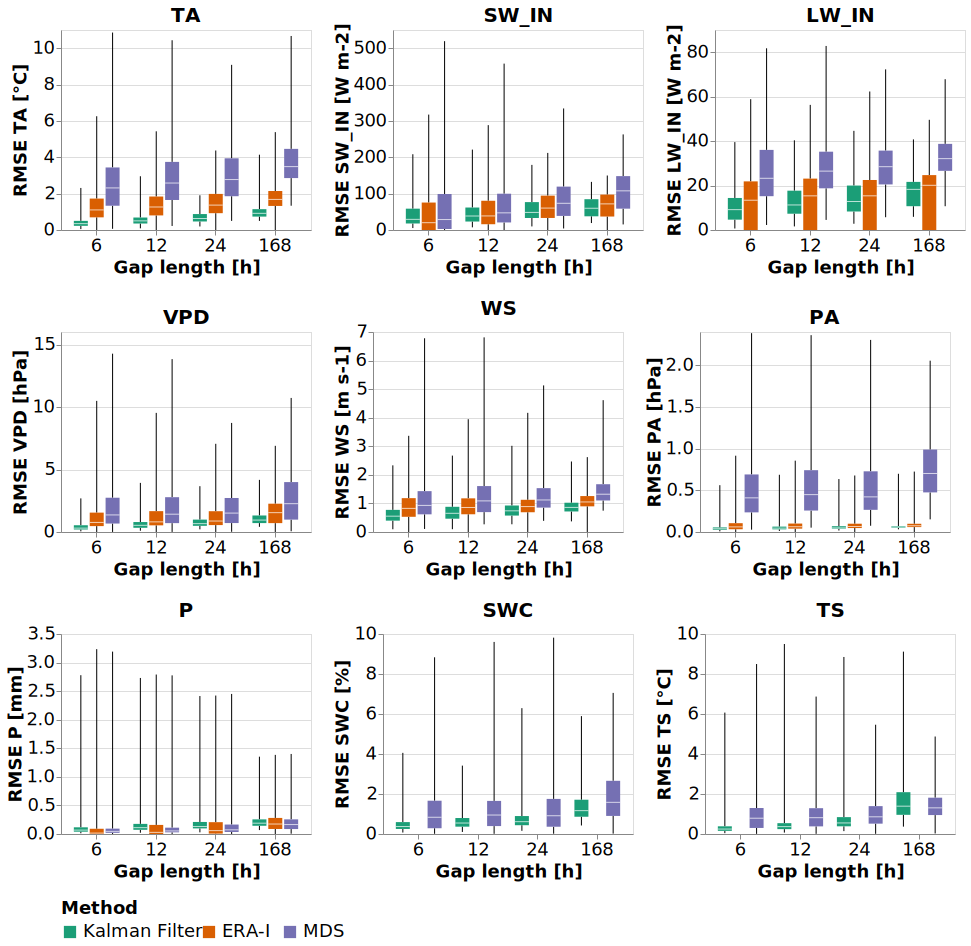
\includegraphics[width=\imgwidth]{the_plot}}
\caption{Box plot to compare Root Mean Square Error(RMSE) for each variable between the different methods: Kalman Filter and the state of the art methods ERA and MDS.  Each box is delimitated by the first and third quartile, the white mark is the median and then vertical lines extend from the minimum to the maximum. For each variable and each gap length 400 artificial gaps has been made only in the variable of interest and the gap imputed using the different methods. The Kalman Filter model has been fine-tuned to each variable. ERA-I imputation is not available for \texttt{TS} and \texttt{SWC}}
\label{fig:the_plot}
\end{figure}

\begin{table}
\centering
\caption{\CapTheTable}
\label{tbl:the_table}
\begin{tabular}{p{2.1cm}l|rr|rr|rr}
\toprule
 &  & \multicolumn{2}{r}{Kalman Filter} & \multicolumn{2}{r}{ERA-I} & \multicolumn{2}{r}{MDS} \\
 & RMSE & mean & std & mean & std & mean & std \\
Variable & Gap &  &  &  &  &  &  \\
\midrule
\multirow[c]{4}{*}{\parbox{2.1cm}{\textbf{TA} [\si{°C}]}} & 6 h & \bfseries 0.405 & 0.258 & 1.347 & 0.998 & 2.713 & 1.897 \\
 & 12 h & \bfseries 0.607 & 0.401 & 1.472 & 0.901 & 2.942 & 1.748 \\
 & 1 day (24 h) & \bfseries 0.741 & 0.368 & 1.530 & 0.800 & 3.013 & 1.611 \\
 & 1 week (168 h) & \bfseries 1.021 & 0.445 & 1.754 & 0.643 & 3.780 & 1.315 \\
\cline{1-8}
\multirow[c]{4}{*}{\parbox{2.1cm}{\textbf{SW\_IN} [\si{W/m^2}]}} & 6 h & \bfseries 44.637 & 40.465 & 49.333 & 66.242 & 63.537 & 85.402 \\
 & 12 h & \bfseries 48.155 & 33.868 & 54.208 & 49.769 & 69.427 & 68.936 \\
 & 1 day (24 h) & \bfseries 56.564 & 30.043 & 65.950 & 40.931 & 86.771 & 59.604 \\
 & 1 week (168 h) & \bfseries 61.583 & 25.740 & 70.224 & 34.883 & 107.384 & 53.606 \\
\cline{1-8}
\multirow[c]{4}{*}{\parbox{2.1cm}{\textbf{LW\_IN} [\si{W/m^2}]}} & 6 h & \bfseries 10.902 & 7.736 & 13.805 & 12.988 & 26.680 & 15.022 \\
 & 12 h & \bfseries 13.422 & 7.735 & 14.767 & 12.585 & 28.085 & 13.457 \\
 & 1 day (24 h) & 14.594 & 7.840 & \bfseries 14.093 & 12.228 & 29.614 & 12.417 \\
 & 1 week (168 h) & 17.063 & 6.425 & \bfseries 16.366 & 11.130 & 32.955 & 8.834 \\
\cline{1-8}
\multirow[c]{4}{*}{\parbox{2.1cm}{\textbf{VPD} [\si{hPa}]}} & 6 h & \bfseries 0.428 & 0.363 & 1.297 & 1.547 & 2.084 & 2.149 \\
 & 12 h & \bfseries 0.661 & 0.505 & 1.265 & 1.289 & 2.137 & 2.096 \\
 & 1 day (24 h) & \bfseries 0.828 & 0.502 & 1.248 & 1.032 & 1.912 & 1.605 \\
 & 1 week (168 h) & \bfseries 1.126 & 0.633 & 1.662 & 1.127 & 2.661 & 1.965 \\
\cline{1-8}
\multirow[c]{4}{*}{\parbox{2.1cm}{\textbf{WS} [\si{m/s}]}} & 6 h & \bfseries 0.617 & 0.317 & 0.912 & 0.508 & 1.136 & 0.783 \\
 & 12 h & \bfseries 0.715 & 0.351 & 0.957 & 0.524 & 1.261 & 0.797 \\
 & 1 day (24 h) & \bfseries 0.802 & 0.343 & 0.949 & 0.447 & 1.276 & 0.609 \\
 & 1 week (168 h) & \bfseries 0.950 & 0.363 & 1.089 & 0.349 & 1.495 & 0.615 \\
\cline{1-8}
\multirow[c]{4}{*}{\parbox{2.1cm}{\textbf{PA} [\si{hPa}]}} & 6 h & \bfseries 0.045 & 0.034 & 0.075 & 0.062 & 0.531 & 0.441 \\
 & 12 h & \bfseries 0.053 & 0.042 & 0.077 & 0.058 & 0.564 & 0.427 \\
 & 1 day (24 h) & \bfseries 0.059 & 0.039 & 0.079 & 0.051 & 0.557 & 0.404 \\
 & 1 week (168 h) & \bfseries 0.066 & 0.048 & 0.084 & 0.054 & 0.773 & 0.384 \\
\cline{1-8}
\multirow[c]{4}{*}{\parbox{2.1cm}{\textbf{P} [\si{mm}]}} & 6 h & 0.134 & 0.274 & \bfseries 0.113 & 0.316 & 0.118 & 0.306 \\
 & 12 h & 0.179 & 0.295 & 0.139 & 0.297 & \bfseries 0.130 & 0.281 \\
 & 1 day (24 h) & 0.206 & 0.254 & 0.166 & 0.288 & \bfseries 0.159 & 0.265 \\
 & 1 week (168 h) & 0.240 & 0.174 & 0.223 & 0.202 & \bfseries 0.215 & 0.197 \\
\cline{1-8}
\multirow[c]{4}{*}{\parbox{2.1cm}{\textbf{SWC} [\si{\%}]}} & 6 h & \bfseries 0.508 & 0.487 & - & - & 1.314 & 1.557 \\
 & 12 h & \bfseries 0.665 & 0.472 & - & - & 1.278 & 1.323 \\
 & 1 day (24 h) & \bfseries 0.779 & 0.641 & - & - & 1.356 & 1.472 \\
 & 1 week (168 h) & \bfseries 1.494 & 0.948 & - & - & 1.948 & 1.488 \\
\cline{1-8}
\multirow[c]{4}{*}{\parbox{2.1cm}{\textbf{TS} [\si{°C}]}} & 6 h & \bfseries 0.341 & 0.432 & - & - & 0.954 & 0.889 \\
 & 12 h & \bfseries 0.534 & 0.784 & - & - & 1.003 & 0.877 \\
 & 1 day (24 h) & \bfseries 0.787 & 0.852 & - & - & 1.078 & 0.857 \\
 & 1 week (168 h) & 1.660 & 1.078 & - & - & \bfseries 1.440 & 0.764 \\
\cline{1-8}
\bottomrule
\end{tabular}
\end{table}


\begin{itemize}
    \item TA: KF good performance and improvement over ERA. For long gaps follows ERA but often better. For reference the accuracy of the thermometer installed at Hainich \cite{noauthor_associated_2020} is 0.1 \si{°C} \cite{noauthor_specification_nodate}.
    \item SW\_IN: KF performance at night is not good, there are negative values up to -50 and then a lot of variation even though should be constant at 0 and the control variable is correct. During the day methods are comparable with often Kalman Filter having the best performance 
    \item LW\_IN KF compare performance ERA. ERA has a much wider range of errors, for some gaps is very good for others is quite worse. MDS is quite bad basically predicting a constant value and the come drastic changes. LW\_IN has a "blocky" behaviour that is correctly predicted by ERA
    \item VPD. KF is better especially for short gaps. MDS not very good miss variation at night (probably due to no change in SW\_IN)
    \item WS has the worse standarized RMSE, a lot of short term variability that no model captures. KF still best results 
    \item PA MDS significantly worse than other methods
    \item P KF worse performance than other methods, but still similar performance
    \item SWC KF has on average a better performance than MDS, especially for short gaps. However, the time series of KF are not very good. The variation in the predicted time series is often much higher than the actual one (Figure \ref{fig:ts_2_0} \ref{fig:ts_2_1} \ref{fig:ts_2_2}). ERA is not available
    \item TS KF has on average a better performance than MDS, especially for short gaps. However, the time series of KF are not very good. The variation in the predicted time series is often much higher than the actual one when there is a small variation in the variable(Figure \ref{fig:ts_2_0} gap length 6h and 12h) conversely is much better when there is variation \ref{fig:ts_2_1} \ref{fig:ts_2_2}), specifically the KF models correctly the increase and decrease in soil temperature even though if the values may not be accurate. ERA is not available
    
\end{itemize}

\begin{figure}
    \centerline{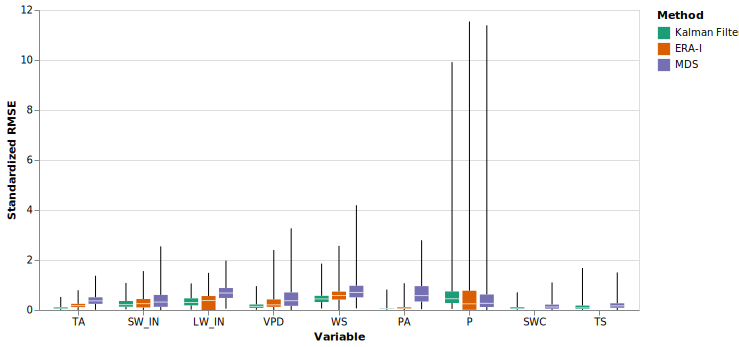
\includegraphics[width=\imgwidth]{the_plot_stand}}
\caption{Box plot to compare Standardized Root Mean Square Error(RMSE) for each variable between the different methods: Kalman Filter and the state of the art methods ERA and MDS. The same data from figure \ref{fig:the_plot} has been aggregated for all gap lengths}
\label{fig:the_plot}
\end{figure}


\begin{table}
\centering
\caption{Comparison of imputation methods using Standardized RMSE. The best method for each gap length is highligthed in bold}
\label{the_table_stand}
\begin{tabular}{p{2.1cm}c|rr|rr|rr}
\toprule
 &  & \multicolumn{2}{r}{KalmanFilter} & \multicolumn{2}{r}{ERA} & \multicolumn{2}{r}{MDS} \\
 & RMSE & mean & std & mean & std & mean & std \\
Variable & Gap [$h$] &  &  &  &  &  &  \\
\midrule
\multirow[c]{4}{*}{\parbox{2.1cm}{\textbf{TA}}} & 6 & \bfseries 0.063 & 0.037 & 0.171 & 0.129 & 0.337 & 0.239 \\
 & 12 & \bfseries 0.087 & 0.052 & 0.176 & 0.110 & 0.367 & 0.209 \\
 & 24 & \bfseries 0.107 & 0.058 & 0.191 & 0.098 & 0.363 & 0.192 \\
 & 168 & \bfseries 0.137 & 0.055 & 0.223 & 0.077 & 0.468 & 0.153 \\
\cline{1-8}
\multirow[c]{4}{*}{\parbox{2.1cm}{\textbf{SW\_IN}}} & 6 & \bfseries 0.229 & 0.211 & 0.258 & 0.337 & 0.329 & 0.435 \\
 & 12 & \bfseries 0.252 & 0.173 & 0.279 & 0.248 & 0.372 & 0.367 \\
 & 24 & \bfseries 0.287 & 0.154 & 0.328 & 0.211 & 0.432 & 0.303 \\
 & 168 & \bfseries 0.299 & 0.121 & 0.337 & 0.168 & 0.519 & 0.258 \\
\cline{1-8}
\multirow[c]{4}{*}{\parbox{2.1cm}{\textbf{LW\_IN}}} & 6 & \bfseries 0.254 & 0.189 & 0.321 & 0.295 & 0.642 & 0.350 \\
 & 12 & \bfseries 0.321 & 0.201 & 0.362 & 0.295 & 0.695 & 0.335 \\
 & 24 & \bfseries 0.355 & 0.194 & 0.367 & 0.295 & 0.682 & 0.282 \\
 & 168 & 0.412 & 0.170 & \bfseries 0.399 & 0.266 & 0.776 & 0.219 \\
\cline{1-8}
\multirow[c]{4}{*}{\parbox{2.1cm}{\textbf{VPD}}} & 6 & \bfseries 0.136 & 0.100 & 0.304 & 0.360 & 0.489 & 0.507 \\
 & 12 & \bfseries 0.194 & 0.133 & 0.289 & 0.286 & 0.467 & 0.458 \\
 & 24 & \bfseries 0.216 & 0.130 & 0.296 & 0.248 & 0.469 & 0.424 \\
 & 168 & \bfseries 0.288 & 0.142 & 0.373 & 0.245 & 0.601 & 0.429 \\
\cline{1-8}
\multirow[c]{4}{*}{\parbox{2.1cm}{\textbf{WS}}} & 6 & \bfseries 0.358 & 0.185 & 0.564 & 0.344 & 0.696 & 0.438 \\
 & 12 & \bfseries 0.440 & 0.197 & 0.593 & 0.325 & 0.758 & 0.465 \\
 & 24 & \bfseries 0.504 & 0.242 & 0.615 & 0.297 & 0.795 & 0.465 \\
 & 168 & \bfseries 0.569 & 0.191 & 0.655 & 0.202 & 0.924 & 0.353 \\
\cline{1-8}
\multirow[c]{4}{*}{\parbox{2.1cm}{\textbf{PA}}} & 6 & \bfseries 0.058 & 0.077 & 0.095 & 0.114 & 0.605 & 0.477 \\
 & 12 & \bfseries 0.068 & 0.070 & 0.094 & 0.085 & 0.710 & 0.520 \\
 & 24 & \bfseries 0.066 & 0.029 & 0.089 & 0.049 & 0.663 & 0.478 \\
 & 168 & \bfseries 0.082 & 0.077 & 0.103 & 0.082 & 0.923 & 0.451 \\
\cline{1-8}
\multirow[c]{4}{*}{\parbox{2.1cm}{\textbf{P}}} & 6 & 0.419 & 0.872 & 0.435 & 1.046 & \bfseries 0.418 & 0.999 \\
 & 12 & 0.435 & 0.784 & 0.438 & 0.924 & \bfseries 0.418 & 0.847 \\
 & 24 & \bfseries 0.537 & 0.827 & 0.553 & 0.955 & 0.545 & 0.935 \\
 & 168 & \bfseries 0.701 & 0.632 & 0.793 & 0.711 & 0.766 & 0.704 \\
\cline{1-8}
\multirow[c]{4}{*}{\parbox{2.1cm}{\textbf{SWC}}} & 6 & \bfseries 0.057 & 0.043 & nan & nan & 0.143 & 0.164 \\
 & 12 & \bfseries 0.069 & 0.053 & nan & nan & 0.146 & 0.163 \\
 & 24 & \bfseries 0.082 & 0.060 & nan & nan & 0.146 & 0.131 \\
 & 168 & \bfseries 0.171 & 0.116 & nan & nan & 0.210 & 0.166 \\
\cline{1-8}
\multirow[c]{4}{*}{\parbox{2.1cm}{\textbf{TS}}} & 6 & \bfseries 0.070 & 0.057 & nan & nan & 0.184 & 0.177 \\
 & 12 & \bfseries 0.108 & 0.088 & nan & nan & 0.186 & 0.172 \\
 & 24 & \bfseries 0.159 & 0.155 & nan & nan & 0.192 & 0.155 \\
 & 168 & \bfseries 0.256 & 0.149 & nan & nan & 0.271 & 0.161 \\
\cline{1-8}
\bottomrule
\end{tabular}
\end{table}



\subsubsection{Example Time series}

\newgeometry{top=.1in}
\begin{figure}
\centerline{\includegraphics[width=\imgwidth]{timeseries_1}}
\caption{Example time series for \texttt{TA, SW\_IN, LW\_IN, VPD, WS}. For each variable, 3 random artificial gap (length 6 hours, 12 hours, 1 week) are imputed using the three methods: Kalman Filter (green), ERA-I (orange), MDS (purple). For the Kalman Filter the shared area show the uncertainty of the prediction $+/- 2 \sigma$. The vertical black line are the start and the beginning of the gap.}
\label{fig:ts_1_0}
\end{figure}
\restoregeometry

\begin{figure}
\centerline{\includegraphics[width=\imgwidth]{timeseries_2}}
\caption{Example time series for \texttt{TA, SW\_IN, LW\_IN, VPD, WS}. For each variable, 3 random artificial gap (length 6 hours, 12 hours, 1 week) are imputed using the three methods: Kalman Filter (green), ERA-I (orange), MDS (purple). For the Kalman Filter the shared area show the uncertainty of the prediction $+/- 2 \sigma$. The vertical black line are the start and the beginning of the gap.}
\label{fig:ts_2_0}
\end{figure}

% \textbf{goal} Show how a Kalman Filter Gap filling looks like and the uncertainty 

% \begin{figure}
% \centerline{\includegraphics[width=6in]{timeseries_1}}
% \caption{Timeseries 1}
% \end{figure}

% \begin{itemize}
%     \item a few sample variables (max 3/4)
%     \item a representative gap length
%     \item manually choose interesting gaps (2-4)
%     \item no gap in other variable
% \end{itemize}

% This is the most intuitive way of looking at gap filling and can select the gaps for highlighting the strengths and weakness of the filter


\subsection{Analysis Kalman Filter}

\subsubsection{Gap Length}

\begin{itemize}
    \item short gaps have a smaller error
    \item then there is a steep increase for gaps up to 24 hours
    \item after 24 hours the is no or little change into the error
    \item the variability on of the error between gaps (std of RMSE) follows a similar partner
    \item P and SWC are an exception from this pattern, with both the mean and std oft the error increasing for gaps longer than a day
\end{itemize}

% \textbf{goal} impact of the gap length on the gap filling
\begin{figure}
\centerline{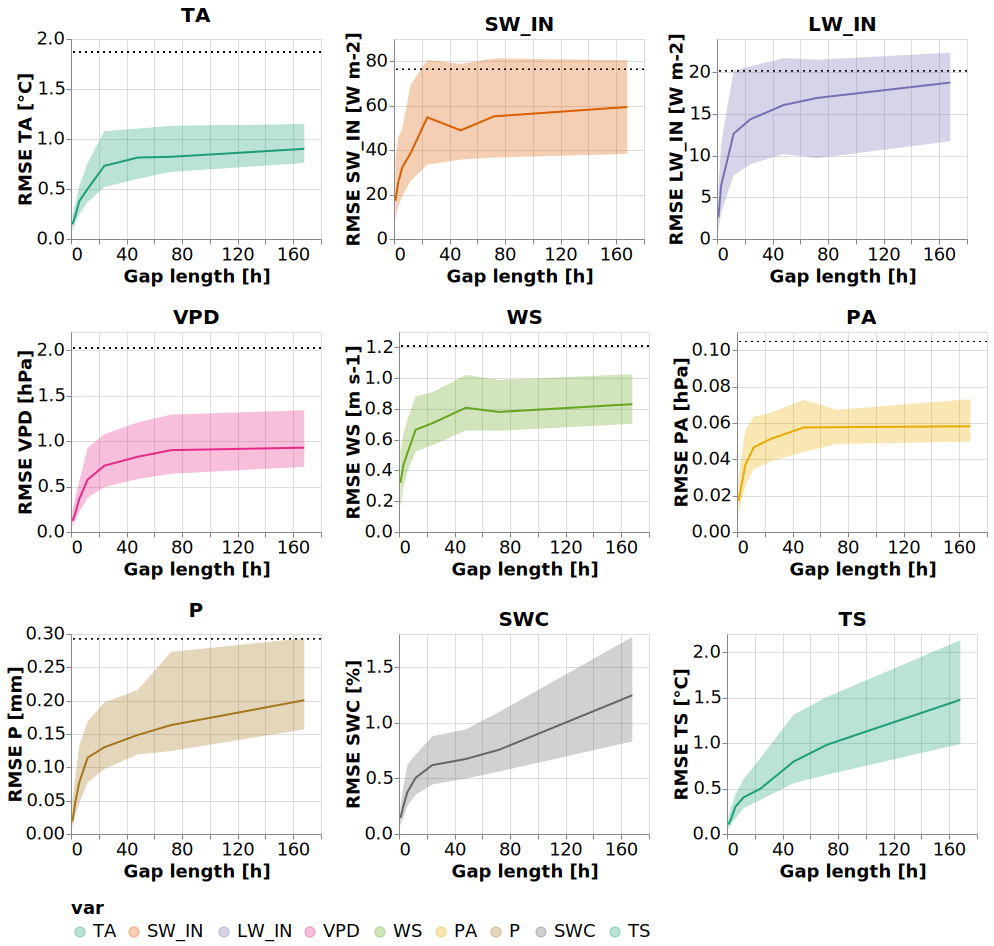
\includegraphics[width=\imgwidth]{gap_len}}
\caption{Gap len}
\label{fig:gap_len}
\end{figure}

\begin{table}
\centering
\caption{RMSE Comparison Kalman filter for different gap lengths}
\label{gap_len}
\begin{tabular}{p{2.1cm}l|cccccccc}
\toprule
 &  & 1 & 3 & 6 & 12 & 24 & 48 & 72 & 168 \\
Variable & RMSE &  &  &  &  &  &  &  &  \\
\midrule
\parbox{2.1cm}{\textbf{TA}} & mean & 0.194 & 0.287 & 0.440 & 0.628 & 0.826 & 0.904 & 0.939 & 0.986 \\
\cline{1-10}
\parbox{2.1cm}{\textbf{SW\_IN}} & mean & 27.869 & 37.737 & 44.486 & 50.090 & 57.306 & 58.099 & 58.938 & 59.045 \\
\cline{1-10}
\parbox{2.1cm}{\textbf{LW\_IN}} & mean & 5.628 & 7.948 & 11.455 & 13.292 & 15.916 & 17.051 & 16.284 & 17.491 \\
\cline{1-10}
\parbox{2.1cm}{\textbf{VPD}} & mean & 0.180 & 0.319 & 0.501 & 0.688 & 0.946 & 0.957 & 1.062 & 1.105 \\
\cline{1-10}
\parbox{2.1cm}{\textbf{WS}} & mean & 0.361 & 0.495 & 0.616 & 0.770 & 0.830 & 0.906 & 0.917 & 0.914 \\
\cline{1-10}
\parbox{2.1cm}{\textbf{PA}} & mean & 0.022 & 0.034 & 0.048 & 0.053 & 0.059 & 0.068 & 0.066 & 0.070 \\
\cline{1-10}
\parbox{2.1cm}{\textbf{P}} & mean & 0.092 & 0.165 & 0.116 & 0.200 & 0.186 & 0.208 & 0.215 & 0.238 \\
\cline{1-10}
\parbox{2.1cm}{\textbf{SWC}} & mean & 0.187 & 0.332 & 0.453 & 0.617 & 0.752 & 0.910 & 0.959 & 1.460 \\
\cline{1-10}
\parbox{2.1cm}{\textbf{TS}} & mean & 0.152 & 0.232 & 0.382 & 0.591 & 0.677 & 0.995 & 1.358 & 1.663 \\
\cline{1-10}
\bottomrule
\end{tabular}
\end{table}


\subsubsection{Gap other variable}

\begin{figure}
\centerline{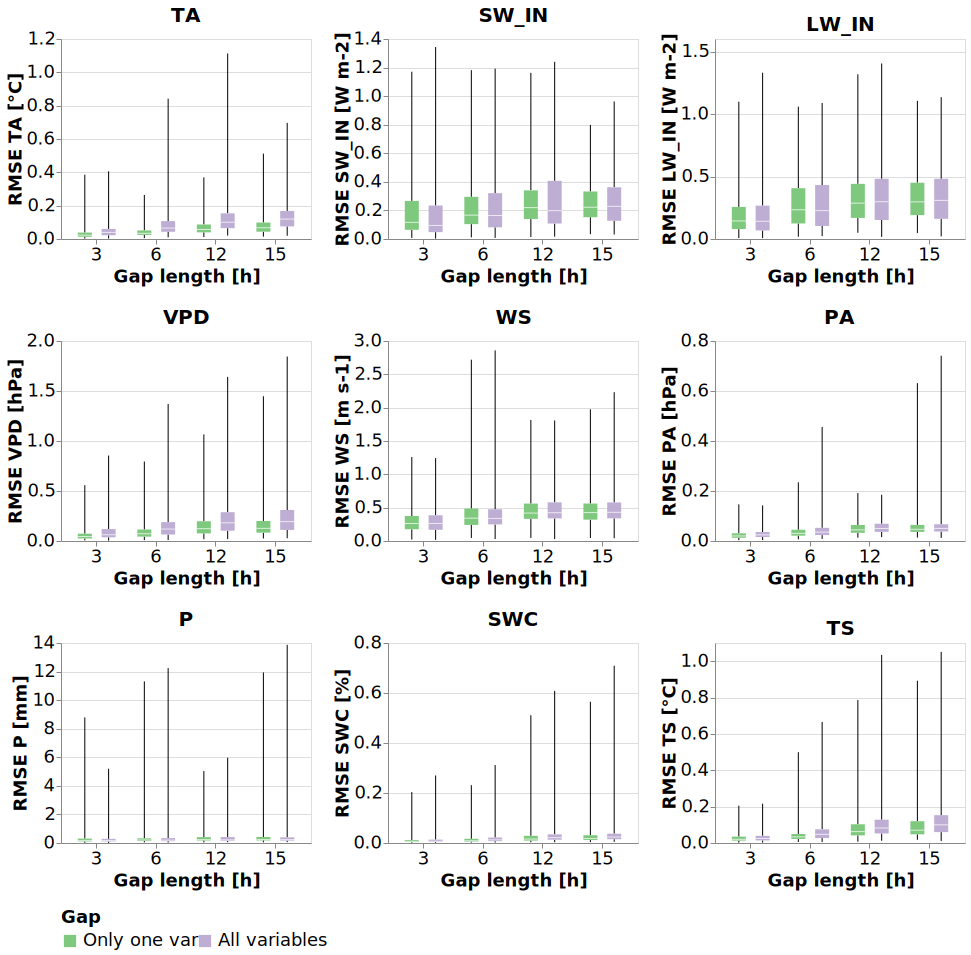
\includegraphics[width=\imgwidth]{gap_single_var}}
\caption{Gap single var}
\label{fig:gap_single_var}
\end{figure}

\begin{table}
\centering
\begin{tabular}{p{2.1cm}c|rr|rr|r}
\toprule
 & Gap & \multicolumn{2}{r}{Only one var} & \multicolumn{2}{r}{All variables} &  \\
 & RMSE Standardized & mean & std & mean & std & diff. \\
Variable & Gap [$h$] &  &  &  &  &  \\
\midrule
\multirow[c]{4}{*}{\parbox{2.1cm}{\textbf{TA}}} & 3 & \bfseries 0.029 & 0.024 & 0.049 & 0.048 & 0.020 \\
 & 6 & \bfseries 0.040 & 0.028 & 0.078 & 0.052 & 0.039 \\
 & 12 & \bfseries 0.073 & 0.050 & 0.129 & 0.083 & 0.056 \\
 & 15 & \bfseries 0.079 & 0.057 & 0.138 & 0.092 & 0.059 \\
\cline{1-7}
\multirow[c]{4}{*}{\parbox{2.1cm}{\textbf{SW\_IN}}} & 3 & \bfseries 0.199 & 0.205 & 0.202 & 0.244 & 0.003 \\
 & 6 & \bfseries 0.222 & 0.171 & 0.228 & 0.215 & 0.006 \\
 & 12 & \bfseries 0.260 & 0.167 & 0.284 & 0.221 & 0.024 \\
 & 15 & \bfseries 0.277 & 0.166 & 0.307 & 0.217 & 0.030 \\
\cline{1-7}
\multirow[c]{4}{*}{\parbox{2.1cm}{\textbf{LW\_IN}}} & 3 & 0.194 & 0.169 & \bfseries 0.187 & 0.174 & -0.007 \\
 & 6 & \bfseries 0.276 & 0.216 & 0.288 & 0.234 & 0.012 \\
 & 12 & \bfseries 0.325 & 0.197 & 0.328 & 0.223 & 0.002 \\
 & 15 & \bfseries 0.337 & 0.188 & 0.345 & 0.212 & 0.008 \\
\cline{1-7}
\multirow[c]{4}{*}{\parbox{2.1cm}{\textbf{VPD}}} & 3 & \bfseries 0.070 & 0.070 & 0.105 & 0.105 & 0.035 \\
 & 6 & \bfseries 0.103 & 0.097 & 0.161 & 0.141 & 0.059 \\
 & 12 & \bfseries 0.155 & 0.116 & 0.233 & 0.193 & 0.078 \\
 & 15 & \bfseries 0.183 & 0.134 & 0.286 & 0.227 & 0.103 \\
\cline{1-7}
\multirow[c]{4}{*}{\parbox{2.1cm}{\textbf{WS}}} & 3 & \bfseries 0.297 & 0.179 & 0.301 & 0.181 & 0.004 \\
 & 6 & \bfseries 0.366 & 0.202 & 0.371 & 0.211 & 0.005 \\
 & 12 & \bfseries 0.460 & 0.242 & 0.468 & 0.248 & 0.009 \\
 & 15 & \bfseries 0.481 & 0.230 & 0.494 & 0.249 & 0.013 \\
\cline{1-7}
\multirow[c]{4}{*}{\parbox{2.1cm}{\textbf{PA}}} & 3 & \bfseries 0.024 & 0.016 & 0.029 & 0.020 & 0.005 \\
 & 6 & \bfseries 0.036 & 0.027 & 0.041 & 0.032 & 0.005 \\
 & 12 & \bfseries 0.057 & 0.074 & 0.064 & 0.091 & 0.007 \\
 & 15 & \bfseries 0.061 & 0.090 & 0.064 & 0.099 & 0.003 \\
\cline{1-7}
\multirow[c]{4}{*}{\parbox{2.1cm}{\textbf{P}}} & 3 & 0.290 & 0.450 & \bfseries 0.283 & 0.460 & -0.007 \\
 & 6 & \bfseries 0.386 & 0.524 & 0.396 & 0.592 & 0.010 \\
 & 12 & \bfseries 0.390 & 0.550 & 0.393 & 0.640 & 0.003 \\
 & 15 & \bfseries 0.442 & 0.675 & 0.449 & 0.767 & 0.008 \\
\cline{1-7}
\multirow[c]{4}{*}{\parbox{2.1cm}{\textbf{SWC}}} & 3 & \bfseries 0.013 & 0.032 & 0.013 & 0.033 & 0.000 \\
 & 6 & \bfseries 0.017 & 0.025 & 0.022 & 0.030 & 0.004 \\
 & 12 & \bfseries 0.026 & 0.034 & 0.032 & 0.036 & 0.006 \\
 & 15 & \bfseries 0.034 & 0.040 & 0.041 & 0.053 & 0.007 \\
\cline{1-7}
\multirow[c]{4}{*}{\parbox{2.1cm}{\textbf{TS}}} & 3 & \bfseries 0.024 & 0.023 & 0.031 & 0.036 & 0.007 \\
 & 6 & \bfseries 0.046 & 0.044 & 0.065 & 0.055 & 0.019 \\
 & 12 & \bfseries 0.083 & 0.088 & 0.106 & 0.112 & 0.023 \\
 & 15 & \bfseries 0.114 & 0.114 & 0.138 & 0.137 & 0.024 \\
\cline{1-7}
\bottomrule
\end{tabular}
\end{table}


\subsubsection{Control variable}

\begin{itemize}
    \item Across all variables the control is helping achieving a better performance
    \item generically the longer the gap the 
    \item the difference varies a lot between variables
    \item PA and SWC have the biggest improvement
    \item little change for P
    \item variability RMSE is higher for absence of control
\end{itemize}

% \textbf{goal} show how the use of the control (ERA-5 data) in the gap is impacting the predictions

% \includegraphics[width=\textwidth]{use_control}

\begin{figure}
\centerline{\includegraphics[width=\imgwidth]{images/use_control.png}}
\caption{Control}
\label{fig:control}
\end{figure}

\begin{table}
\centering
\caption{RMSE Comparison Kalman filter with and without control variable. The best result for each for each gap length is highligthed in bold}
\label{control}
\begin{tabular}{p{2.1cm}c|rr|rr|r}
\toprule
 & type & \multicolumn{2}{r}{Use Control} & \multicolumn{2}{r}{No Control} &  \\
 & RMSE Standardized & mean & std & mean & std & diff. \\
Variable & Gap [$h$] &  &  &  &  &  \\
\midrule
\multirow[c]{4}{*}{\parbox{2.1cm}{\textbf{TA} [\si{°C}]}} & 6 & 0.158 & 0.107 & \bfseries 0.118 & 0.066 & 0.040 \\
 & 12 & \bfseries 0.185 & 0.097 & 0.194 & 0.110 & 0.008 \\
 & 24 & \bfseries 0.254 & 0.133 & 0.274 & 0.164 & 0.021 \\
 & 168 & 0.267 & 0.065 & \bfseries 0.249 & 0.104 & 0.018 \\
\cline{1-7}
\multirow[c]{4}{*}{\parbox{2.1cm}{\textbf{SW\_IN} [\si{W/m^2}]}} & 6 & \bfseries 0.289 & 0.179 & 0.347 & 0.217 & 0.058 \\
 & 12 & \bfseries 0.345 & 0.177 & 0.524 & 0.285 & 0.179 \\
 & 24 & \bfseries 0.408 & 0.167 & 0.570 & 0.267 & 0.162 \\
 & 168 & \bfseries 0.435 & 0.124 & 0.597 & 0.232 & 0.161 \\
\cline{1-7}
\multirow[c]{4}{*}{\parbox{2.1cm}{\textbf{LW\_IN} [\si{W/m^2}]}} & 6 & 0.382 & 0.222 & \bfseries 0.300 & 0.179 & 0.082 \\
 & 12 & \bfseries 0.449 & 0.228 & 0.465 & 0.183 & 0.016 \\
 & 24 & \bfseries 0.487 & 0.190 & 0.534 & 0.185 & 0.047 \\
 & 168 & \bfseries 0.569 & 0.141 & 0.643 & 0.147 & 0.074 \\
\cline{1-7}
\multirow[c]{4}{*}{\parbox{2.1cm}{\textbf{VPD} [\si{hPa}]}} & 6 & 0.212 & 0.122 & \bfseries 0.202 & 0.198 & 0.009 \\
 & 12 & \bfseries 0.259 & 0.126 & 0.270 & 0.172 & 0.011 \\
 & 24 & \bfseries 0.373 & 0.184 & 0.383 & 0.332 & 0.009 \\
 & 168 & \bfseries 0.378 & 0.127 & 0.396 & 0.155 & 0.018 \\
\cline{1-7}
\multirow[c]{4}{*}{\parbox{2.1cm}{\textbf{WS} [\si{m/s}]}} & 6 & \bfseries 0.404 & 0.210 & 0.425 & 0.255 & 0.021 \\
 & 12 & \bfseries 0.544 & 0.194 & 0.616 & 0.290 & 0.071 \\
 & 24 & \bfseries 0.617 & 0.230 & 0.817 & 0.328 & 0.200 \\
 & 168 & \bfseries 0.695 & 0.208 & 0.900 & 0.293 & 0.206 \\
\cline{1-7}
\multirow[c]{4}{*}{\parbox{2.1cm}{\textbf{PA} [\si{hPa}]}} & 6 & \bfseries 0.123 & 0.090 & 0.146 & 0.087 & 0.024 \\
 & 12 & \bfseries 0.164 & 0.105 & 0.333 & 0.206 & 0.170 \\
 & 24 & \bfseries 0.179 & 0.065 & 0.655 & 0.387 & 0.476 \\
 & 168 & \bfseries 0.224 & 0.110 & 0.928 & 0.422 & 0.704 \\
\cline{1-7}
\multirow[c]{4}{*}{\parbox{2.1cm}{\textbf{P} [\si{mm}]}} & 6 & \bfseries 0.440 & 0.888 & 0.635 & 1.561 & 0.195 \\
 & 12 & 0.648 & 1.766 & \bfseries 0.543 & 0.627 & 0.105 \\
 & 24 & \bfseries 0.501 & 0.687 & 0.767 & 1.462 & 0.266 \\
 & 168 & \bfseries 0.793 & 0.707 & 0.822 & 0.751 & 0.029 \\
\cline{1-7}
\multirow[c]{4}{*}{\parbox{2.1cm}{\textbf{SWC} [\si{\%}]}} & 6 & 0.201 & 0.127 & \bfseries 0.122 & 0.090 & 0.078 \\
 & 12 & 0.345 & 0.206 & \bfseries 0.286 & 0.164 & 0.058 \\
 & 24 & 0.627 & 0.312 & \bfseries 0.495 & 0.252 & 0.131 \\
 & 168 & 0.812 & 0.390 & \bfseries 0.741 & 0.308 & 0.071 \\
\cline{1-7}
\multirow[c]{4}{*}{\parbox{2.1cm}{\textbf{TS} [\si{°C}]}} & 6 & 0.168 & 0.160 & \bfseries 0.132 & 0.090 & 0.035 \\
 & 12 & 0.230 & 0.139 & \bfseries 0.197 & 0.116 & 0.033 \\
 & 24 & 0.314 & 0.187 & \bfseries 0.264 & 0.197 & 0.051 \\
 & 168 & 0.358 & 0.136 & \bfseries 0.348 & 0.166 & 0.010 \\
\cline{1-7}
\bottomrule
\end{tabular}
\end{table}


\subsubsection{Generic model}

\begin{figure}
\centerline{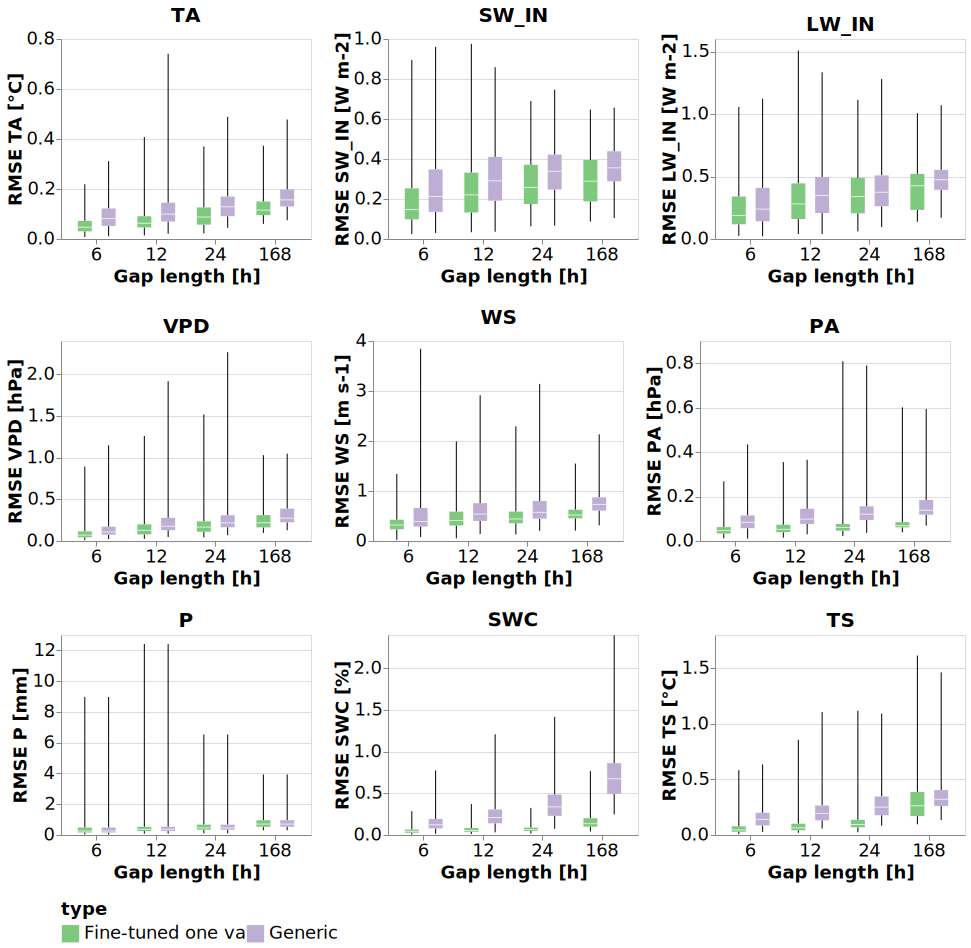
\includegraphics[width=\imgwidth]{images/generic.png}}
\caption{Generic}
\label{fig:generic}
\end{figure}

\begin{table}
\centering
\begin{tabular}{p{2.1cm}c|rr|rr|r}
\toprule
 & type & \multicolumn{2}{r}{Generic} & \multicolumn{2}{r}{Finetuned one var} &  \\
 & RMSE Standardized & std & mean & std & mean & diff. \\
Variable & Gap [$h$] &  &  &  &  &  \\
\midrule
\multirow[c]{4}{*}{\parbox{2.1cm}{\textbf{TA} [\si{°C}]}} & 6 & 0.099 & 0.161 & \bfseries 0.046 & 0.065 & 0.096 \\
 & 12 & 0.112 & 0.210 & \bfseries 0.042 & 0.081 & 0.129 \\
 & 24 & 0.106 & 0.225 & \bfseries 0.061 & 0.112 & 0.113 \\
 & 168 & 0.099 & 0.274 & \bfseries 0.060 & 0.136 & 0.138 \\
\cline{1-7}
\multirow[c]{4}{*}{\parbox{2.1cm}{\textbf{SW\_IN} [\si{W/m^2}]}} & 6 & 0.234 & 0.302 & \bfseries 0.225 & 0.260 & 0.042 \\
 & 12 & 0.220 & 0.374 & \bfseries 0.200 & 0.275 & 0.099 \\
 & 24 & 0.185 & 0.420 & \bfseries 0.148 & 0.285 & 0.135 \\
 & 168 & 0.146 & 0.453 & \bfseries 0.115 & 0.294 & 0.158 \\
\cline{1-7}
\multirow[c]{4}{*}{\parbox{2.1cm}{\textbf{LW\_IN} [\si{W/m^2}]}} & 6 & \bfseries 0.216 & 0.376 & 0.219 & 0.330 & 0.046 \\
 & 12 & 0.331 & 0.477 & \bfseries 0.227 & 0.365 & 0.112 \\
 & 24 & \bfseries 0.196 & 0.531 & 0.200 & 0.370 & 0.161 \\
 & 168 & \bfseries 0.154 & 0.545 & 0.162 & 0.396 & 0.149 \\
\cline{1-7}
\multirow[c]{4}{*}{\parbox{2.1cm}{\textbf{VPD} [\si{hPa}]}} & 6 & 0.122 & 0.223 & \bfseries 0.072 & 0.126 & 0.096 \\
 & 12 & \bfseries 0.117 & 0.250 & 0.129 & 0.184 & 0.066 \\
 & 24 & \bfseries 0.132 & 0.327 & 0.156 & 0.269 & 0.058 \\
 & 168 & 0.151 & 0.391 & \bfseries 0.148 & 0.273 & 0.118 \\
\cline{1-7}
\multirow[c]{4}{*}{\parbox{2.1cm}{\textbf{WS} [\si{m/s}]}} & 6 & 0.272 & 0.417 & \bfseries 0.184 & 0.363 & 0.055 \\
 & 12 & 0.291 & 0.590 & \bfseries 0.189 & 0.409 & 0.180 \\
 & 24 & \bfseries 0.222 & 0.598 & 0.254 & 0.537 & 0.061 \\
 & 168 & 0.243 & 0.778 & \bfseries 0.197 & 0.573 & 0.206 \\
\cline{1-7}
\multirow[c]{4}{*}{\parbox{2.1cm}{\textbf{PA} [\si{hPa}]}} & 6 & 0.077 & 0.110 & \bfseries 0.031 & 0.049 & 0.061 \\
 & 12 & 0.089 & 0.164 & \bfseries 0.031 & 0.065 & 0.099 \\
 & 24 & 0.090 & 0.195 & \bfseries 0.035 & 0.070 & 0.125 \\
 & 168 & 0.085 & 0.219 & \bfseries 0.045 & 0.078 & 0.142 \\
\cline{1-7}
\multirow[c]{4}{*}{\parbox{2.1cm}{\textbf{P} [\si{mm}]}} & 6 & \bfseries 0.634 & 0.325 & 0.636 & 0.371 & 0.045 \\
 & 12 & 0.873 & 0.563 & \bfseries 0.769 & 0.482 & 0.081 \\
 & 24 & 0.906 & 0.531 & \bfseries 0.678 & 0.522 & 0.009 \\
 & 168 & 0.731 & 0.735 & \bfseries 0.502 & 0.633 & 0.102 \\
\cline{1-7}
\multirow[c]{4}{*}{\parbox{2.1cm}{\textbf{SWC} [\si{\%}]}} & 6 & 0.126 & 0.212 & \bfseries 0.038 & 0.055 & 0.157 \\
 & 12 & 0.200 & 0.337 & \bfseries 0.037 & 0.063 & 0.274 \\
 & 24 & 0.290 & 0.586 & \bfseries 0.070 & 0.090 & 0.495 \\
 & 168 & 0.345 & 0.782 & \bfseries 0.104 & 0.180 & 0.601 \\
\cline{1-7}
\multirow[c]{4}{*}{\parbox{2.1cm}{\textbf{TS} [\si{°C}]}} & 6 & 0.117 & 0.156 & \bfseries 0.065 & 0.076 & 0.081 \\
 & 12 & 0.130 & 0.238 & \bfseries 0.078 & 0.100 & 0.139 \\
 & 24 & 0.176 & 0.292 & \bfseries 0.106 & 0.150 & 0.142 \\
 & 168 & 0.174 & 0.377 & \bfseries 0.154 & 0.257 & 0.120 \\
\cline{1-7}
\bottomrule
\end{tabular}
\end{table}




\section{Discussion}

% \subsection{Comparison other methods}

% \begin{itemize}
%     \item Kalman Filter works much better than MDS as it can use observation before/after
%     \item overall low correlation between meteo variables -> MDS is limited
%     \item more precise than ERA as uses local conditions
%     \item problem with precipitation
%     \item SW IN poor performance?
% \end{itemize}

% \subsection{Kalman Filter Components}

% \begin{itemize}
%     \item as expected the longer gap length the worse the performance
%     \item the standard deviation of the increases with gap len
% \end{itemize}

% \begin{itemize}
%     \item the presence of other variables in the gap doesn't help a lot for gap filling
%     \item exception is TA and LW IN, which have higher correlation
%     \item control ?
% \end{itemize}


% \subsection{Impact of numerical stability}

% \begin{itemize}
%     \item max gap len is 15 hours model can be trained
%     \item Kalman filter is a local model, so for long gaps can't really use it
%     \item still need to work to improve numerical stability which should make this better (see appendix)
% \end{itemize}


\subsection{Future steps}

\subsubsection{data}
\begin{itemize}
    \item train model for different sites and see difference between sites
    \item use ERA-5 Land data
\end{itemize}

\subsubsection{Gap filling quality assessment}

\begin{itemize}
    \item can train with more realistic gaps properties (length/other variables missing/time of day)
    \item better analysis of gaps in fluxnet
\end{itemize}

\subsubsection{Model improvement}

\begin{itemize}
\item numerical stability
\item make a model to predict the parameters of the Kalman Filter depending on the conditions
\item use Neural Network to process control variable
\item training and understand variables that are weird
\item include uncertainty of observations in the model
\item high variability ERA data error between sites
\end{itemize}



\section{Conclusions}

\begin{itemize}
    \item Kalman Filter from preliminary results have the potential to improve imputation
    \item lower variability 
    \item on all tested variables smaller or comparable error than other methods, but P
    \item provide interpretable uncertainty
    \item still work needs to be done for model developement and understand the filter performance in different conditions
    \item robust assessment of performance in real life conditions and test different sites
\end{itemize}

\section*{References}

\printbibliography

\appendix

\FloatBarrier


\section{Additional Results}

\subsection{Gap length distribution in FLUXNET}
\begin{figure}
\centerline{\includegraphics[width=\imgwidth]{gap_len_dist}}
\caption{FLUXNET gap len}
\label{fig:gap_len_dist}
\end{figure}
\begin{figure}
\centerline{\includegraphics[width=\imgwidth]{gap_len_dist_small}}
\caption{FLUXNET gap len less than a week}
\label{fig:gap_len_dist_small}
\end{figure}

\subsection{Additional Timeseries}

\begin{figure}
\centerline{\includegraphics[width=\imgwidth]{timeseries_1_1}}
\caption{Timeseries 1}
\label{fig:ts_1_1}
\end{figure}

\begin{figure}
\centerline{\includegraphics[width=\imgwidth]{timeseries_2_1}}
\caption{Timeseries 1}
\label{fig:ts_2_1}
\end{figure}

\begin{figure}
\centerline{\includegraphics[width=\imgwidth]{timeseries_1_2}}
\caption{Timeseries 1}
\label{fig:ts_1_2}
\end{figure}

\begin{figure}
\centerline{\includegraphics[width=\imgwidth]{timeseries_2_2}}
\caption{Timeseries 1}
\label{fig:ts_2_2}
\end{figure}

\section{Comparison Standard Square Root Kalman Filter}

\subsection{Numerical Stability}

\begin{figure}
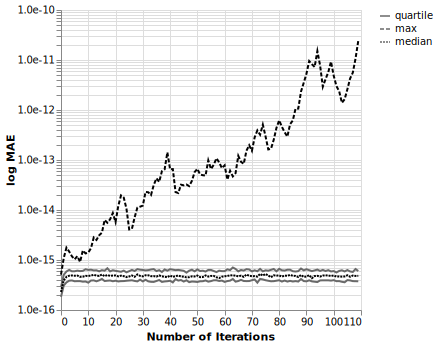
\includegraphics[width=\textwidth]{numerical_stability}
 \caption{Comparison of standard Kalman Filter implementation and Square Root Filter. For 100 times the filter has been initialized with random parameters (drawn from a uniform distribution range 0-1) and then filtered 62 observations. At each filter iteration calculated the Mean Absolute Error (MAE) between the state covariance from the standard filter and the square root filter. The plot shows the median, 1 and 3 quartile and the maximum of the MAE across the 100 samples. You can see that usually the two filter implementations agree, but for a few parameters combinations the error is growing with the number of iterations of the filter suggesting a numerical stability issue. After 62 iterations the standard filter crashes because the covariance is not positive definite anymore. The initial bigger error can be explained by the slightly different initial state covariance.}
\end{figure}


% \section{Detailed Notation}

% \begin{itemize}
% \item $t$  Number of time steps
% \item observations
% \begin{itemize}
%     \item $n$  Number of variables observed
%     \item $y_{:,t}$ or $y_t$ vector of all the $n$ variables at time $t$, $\in \mathbb{R}^n $
%     \item $y_{n,:}$ vector of the $n$th variable at for time steps in $t$, $\in \mathbb{R}^T$
%     \item $y_{n,t}$ $n$th variable at time $t$, $\in \mathbb{R}$ 
%     \item $Y_M = [x_{:,1}, ... x_{:, t}]$ Matrix with all the $n$ variables at all time steps, $\in \mathbb{R}^{n \times t}$ 
%     \item $Y$ is a vector obtained by "flattening" $X_M$, by putting next to each other all variable at time $t$, $\in \mathbb{R}^{(n \cdot t)}$
%     \item $y^{ng}_t$ vector of variable that are not missing (ng = not gap)) at time $t$, $\in \mathbb{R}^{n_{ng}}$. Note at different times the shape of this vector can change
%     \item $Y^{ng}$ all observations
% \end{itemize}

% \item Latent state
% \begin{itemize}
%     \item $k$  Number of variables in latent state
%     \item $x_{:,t}$ or $x_t$ vector of all the $k$ state variables at time $t$, $\in \mathbb{R}^k $
%     \item $x_{k,:}$ vector of the $k$th variable at for time steps in $t$, $\in \mathbb{R}^t$
%     \item $x_{k,t}$ $k$th variable at time $t$, $\in \mathbb{R}$ 
%     \item $X_M = [x_{:,1}, ... x_{:, t}]$ Matrix with all the $k$ variables at all time steps, $\in \mathbb{R}^{k \times t}$ 
%     \item $X$ is a vector obtained by "flattening" $X_M$, by putting next to each other all variable at time $t$, $\in \mathbb{R}^{(k \cdot t)}$
% \end{itemize}

% \end{itemize}

\end{document}

